\documentclass[a4paper, 12pt]{report}
\usepackage{cmap}
\usepackage{amssymb}
\usepackage{amsmath}
\usepackage{graphicx}
\usepackage{float}
\usepackage{wrapfig}
\usepackage{amsthm}
\usepackage{setspace}
\usepackage[T2A]{fontenc}
\usepackage[utf8]{inputenc}
\usepackage[normalem]{ulem}
\usepackage[left=2cm,right=2cm, top=2cm,bottom=2cm,bindingoffset=0cm]{geometry}
\usepackage[english,russian]{babel}
\usepackage[unicode]{hyperref}
\newenvironment{Proof} % имя окружения
{\par\noindent{$\blacklozenge$}} % команды для \begin
{\hfill$\scriptstyle\boxtimes$}
\newenvironment{examp} % имя окружения
{\par\noindent{\textbf{\textsc{Пример:}}}} % команды для \begin
{\hfill$\scriptstyle\Box$}
\usepackage{textcomp}
\title{\textbf{\Huge{Аналитическая геометрия\\ и\\ Основы высшей алгебры}}\\Конспект по 1 семестру факультета прикладной математики и информатики\\(лектор: Б. Б. Комраков)}

\date{}
\begin{document}
	\maketitle
	\tableofcontents{}
	
	
	\part{Аналитическая геометрия}
	
	
	
	
	\chapter{Уравнение плоскости и прямой в пространстве.}
	\section{Уравнение плоскости.}
	$\bullet$ \textit{\textbf{Нормальным вектором плоскости} называется ненулевой вектор, перпендикулярный плоскости.} \\\\
	Рассмотрим некоторую плоскость П, проходящую через т. $M_0 (x_0, y_0, z_0)$ $\perp$ $n(A, B, C).$ \\ т. $M(x, y, z)$ $\in$ П $\Longleftrightarrow$ $\overrightarrow{M M_0}$ $\perp$ $n$ $\Longleftrightarrow$ $\overrightarrow{M_0 M}$ $\cdot$ $n$ = $0$.\\\\
	$\overrightarrow{M M_0}$$(x - x_0, y - y_0, z - z_0)$, \\ 
	$M_0$ $\in$ П $\Longleftrightarrow$ \textit{$A(x - x_0) + B(y - y_0) + C(z - z_0) = 0$} --- $\begin{matrix} \textit{\textbf{уравнение плоскости, проходящей}} \\ \textit{\textbf{через $\overrightarrow{M M_0} \ \perp n$ }} 
	\end{matrix}.$ \\\\
	$M$ $\in$ П $\Longleftrightarrow$ $A(x - x_0) + B(y - y_0) + C(z - z_0) = 0$ \\
	$Ax + By +Cz - \underbrace{A x_0 - B y_0 - C z_0}_{D = -A x_0 - B y_0 - C z_0} = 0$, тогда: \\\\
	\fbox{$Ax + By + Cz + D = 0, \ A^2 + B^2 + C^2 \not= 0$} --- \textit{\textbf{общее уравнение плоскости}}.
	\newtheorem*{t14_1}{Теорема}\begin{t14_1} \end{t14_1}
	\begin{enumerate}
		\item \textit{Любая плоскость может быть задана общим уравнением.}
		\item \textit{В ДПСК любое общее уравнение определяет плоскость.}
	\end{enumerate}
	\newtheorem*{t14_2}{Теорема} \begin{t14_2} Пусть $\text{П}_1$ : $A_1 x + B_1 y + C_1 z + D_1 = 0$, $\text{П}_2$ : $A_2 x + B_2 y + C_2 z + D_2 = 0$. \end{t14_2} 
	\begin{itemize}
		\item \textit{если $\text{П}_1$ = $\text{П}_2$, то $\exists \lambda \in \mathbb{R} : \lambda = \dfrac{A_1}{A_2} = \dfrac{B_1}{B_2} = \dfrac{C_1}{C_2} = \dfrac{D_1}{D_2} $}.
		\item \textit{если $\text{П}_1$ \ $\parallel$ $\text{П}_2$\ $\Longleftrightarrow n_1 \parallel n_2 \ \Longleftrightarrow A_1 = \lambda A_2, \ B_1 = \lambda B_2, \ C_1 = \lambda C_2, \ D_1 \not= \lambda D_2$}.
		\item \textit{если $\text{П}_1$ \ $\perp$ $\text{П}_2$\ $\Longleftrightarrow n_1 \perp n_2 \ \Longleftrightarrow A_1 A_2 + B_1 B_2 + C_1 C_2 = 0$}.
		\item \textit{$cos(\text{П}_1, \text{П}_2) = cos(n_1, n_2) = \dfrac{A_1 A_2 + B_1 B_2 + C_1 C_2}{\sqrt{A_1^2 + B_1^2 + C_1^2} \cdot \sqrt{A_2^2 + B_2^2 + C_2^2}}$}.
	\end{itemize}
	$\bullet$ \textit{\textbf{Общее уравнение} плоскости называется \textbf{полным}, если все его коэффициенты отличны от 0, но если хотя бы один из коэффициентов равен 0, то называется \textbf{неполным}}. \\\\
	Пусть $Ax + By + Cz + D = 0$ --- полное общее уравнение. Перенесем $D$ и разделим:
	\begin{center}
		$\dfrac{Ax}{-D}$ + $\dfrac{By}{-D}$ + $\dfrac{Cz}{-D}$ = 1 $\Rightarrow$ $\dfrac{x}{\dfrac{-D}{A}}$ + $\dfrac{y}{\dfrac{-D}{B}}$ + $\dfrac{z}{\dfrac{-D}{C}}$ = 1 (заменяем: $\dfrac{-D}{A}$ = $a$, $\dfrac{-D}{B}$ = $b$, $\dfrac{-D}{C}$ = $c$) $\Rightarrow$ $\dfrac{x}{a} + \dfrac{y}{b} + \dfrac{z}{c} = 1$ --- \textit{\textbf{уравнение плоскости в отрезках}}.
	\end{center}
	Пусть П --- произвольная плоскость, $n$ --- единичный вектор и имеет координаты $n(cos \alpha, cos \beta, cos \gamma)$, где $\alpha$ = $\angle (n, Ox)$, $\beta$ = $\angle (n, Oy)$, $\gamma$ = $\angle (n, Oz)$ \\\\
	$x \cdot cos \alpha + y \cdot cos \beta + z \cdot cos \gamma - p = 0$ --- $\begin{matrix} \textit{\textbf{нормальное уравнение плоскости}} \end{matrix}$ \\\\
	$\bullet$ \textit{\textbf{Отклонением} $\delta(M, $П$)$ называется число, равное}
	$\delta(M, \text{П}) =  \begin{cases}
		\rho(M, \text{П}) = \overrightarrow{M' M} \ \upuparrows n \\
		-\rho(M, \text{П}), \overrightarrow{M' M} \ \uparrow\downarrow n 
	\end{cases} \Rightarrow \rho(M, \text{П}) = |\delta(M, \text{П})|$. \\
	\newtheorem*{t14_3}{Теорема} \begin{t14_3} Если $x$$\cdot$cos$\alpha$ + $y$$\cdot$cos$\beta$ + $z$$\cdot$cos$\gamma$ - $p$ = 0 --- нормальное уравнение плоскости П, то отношение т.$M_0(x_0, y_0, z_0)$ до плоскости П равняется: \end{t14_3} 
	\begin{center}
		$\delta(M_0, \text{П}) = \ x_0 \cdot cos \alpha + y_0 \cdot cos \beta + z_0 \cdot cos \gamma  - p$ \\
		$\rho(M_0, \text{П}) = |\delta(M_0, \text{П})|$
	\end{center}
	Стоит принять во внимание, что $cos^2 \alpha + cos^2 \beta + cos^2 \gamma$  = 1. \\\\
	Нормальное уравнение можно построить из общего уравнения, домножив его на \textbf{нормирующий множитель} :
	\begin{center}
		$\lambda$ = $\pm$ $\dfrac{1}{\sqrt{A^2 + B^2 + C^2}}$
	\end{center}
	Пусть плоскость П проходит через т.$M_0(x_0, y_0, z_0)$ параллельно двум неколлениарным векторам $a(a_1, a_2, a_3)$ и $b(b_1, b_2, b_3)$. \\\\
	$M(x, y, z)$ $\in$ П $\Longleftrightarrow$ $\overrightarrow{M_0 M}$, $a, b$ --- компланарны ($\overrightarrow{M_0 M}$ $\cdot$ $a$ $\cdot$ $b$ = 0) \\ $\overrightarrow{M M_0}$$(x - x_0, y - y_0, z - z_0)$ \\\\
	$\begin{vmatrix} x - x_0 && y - y_0 && z - z_0 \\ a_1 && a_2 && a_3 \\ b_1 && b_2 && b_3 \end{vmatrix}$ = 0 --- $\begin{matrix} \textit{\textbf{уравнение плоскости, проходящей через точку}} \\ \textit{\textbf{и два направляющих вектора}}  \end{matrix}$ \\\\
	Если плоскость П проходит через 3 точки, не лежащие на одной прямой $M_0(x_0, y_0, z_0)$, $M_1(x_1, y_1, z_1)$, $M_2(x_2, y_2, z_2)$, то в качестве неколлинеарных векторов, параллельных плоскости, можно взять 
	$a$ = $\overrightarrow{M_0 M_1}$ и $b$ = $\overrightarrow{M_0 M_2}$ и тогда уравнение примет вид:
	\begin{center}
		$\begin{vmatrix} x - x_0 && y - y_0 && z - z_0 \\ x_1 - x_0 && y_1 - y_0 && z_1 - z_0 \\ x_2 - x_0 && y_2 - y_0 && z_2 - z_0  \end{vmatrix}$ = 0 --- $\begin{matrix} \textit{\textbf{уравнение плоскости, проходящей через 3}} \\ \textit{\textbf{точки}} \end{matrix}$
	\end{center}
	Т.к. вектор $a(a_1, a_2, a_3)$ $\nparallel$ $b(b_1, b_2, b_3)$, П $\parallel$ $a$ и П $\parallel$ $b$,  и  то векторы $a$ и $b$ на плоскости П образуют базис $\Rightarrow$ любой вектор, параллельный плоскости, в том числе и $\overrightarrow{M_0 M}$, если т.$M$ $\in$ плоскости, может быть разложен по этому базису, т.е. представим в виде:
	\begin{center}
		$M_0 M$ = $t \cdot a$ + $s \cdot b$, \hspace{0.3 cm} $t, s$ $\in$ $R$ $\Rightarrow$ \\
	\end{center}
	$\begin{cases}
		x - x_0 = t \cdot a_1 + s \cdot b_1, \\
		y - y_0 = t \cdot a_2 + s \cdot b_2, \\
		z - z_0 = t \cdot a_3 + s \cdot b_3.
	\end{cases} \Rightarrow
	\begin{cases}
		x = x_0 + t \cdot a_1 + s \cdot b_1, \\
		y = y_0 + t \cdot a_2 + s \cdot b_2, \\
		z = z_0 + t \cdot a_3 + s \cdot b_3.
	\end{cases}
	--- \begin{matrix} \textit{\textbf{параметрическое уравнение}} \\ \textit{\textbf{плоскости}} \end{matrix}$ \\\\
	$\bullet$ \textit{\textbf{Пучок плоскостей} --- совокупность всех плоскостей, проходящих через прямую $\Delta$, причем $\Delta$ --- ось пучка плоскостей.} \\
	\newtheorem*{t14_4}{Теорема} \begin{t14_4} Пусть $\begin{cases}
			\text{П}_1 : A_1 x + B_1 y + C_1 z + D_1 = 0, \\
			\text{П}_2 : A_2 x + B_2 y + C_2 z + D_2 = 0
		\end{cases}$, $\Delta$ $\in \text{П}_1, \text{П}_2$, тогда \\ $\alpha (A_1 x + B_1 y + C_1 z + D_1) + \beta(A_2 x + B_2 y + C_2 z + D_2) = 0$ --- плоскость, проходящая через $\Delta$, причем $\alpha^2 + \beta^2 \not= 0$. \end{t14_4} 
	$\bullet$ \textit{Множество всех плоскостей, проходящих через одну и ту же точку, называется \textbf{связкой}.} \\\\
	Пусть $M_0 (x_0, y_0, z_0)$ --- точка связки с центром, тогда уравнение связки выглядит следующим образом : $A(x - x_0) + B(y - y_0) + C(z - z_0) + D = 0$, причем $A^2 + B^2 + C^2 + D^2 \not= 0$. 
	
	
	
	
	\section{Уравнение прямой в пространстве.}
	$\text{Пусть } \Delta $ --- $\text{прямая}, M_0(x_0, y_0, z_0), M(x, y, z) $ --- $ \text{различные точки, при этом } M_0 \in \Delta, a(a_1, a_2, a_3) -\text{вектор, параллельный прямой } \Delta$ (направляющий вектор). Тогда $a \parallel M_0M \Leftrightarrow M \in \Delta \Leftrightarrow \exists t \in R:$ $$\overrightarrow{M_0M} = ta. \eqno(1)$$
	\begin{figure}[h]
		\centering
		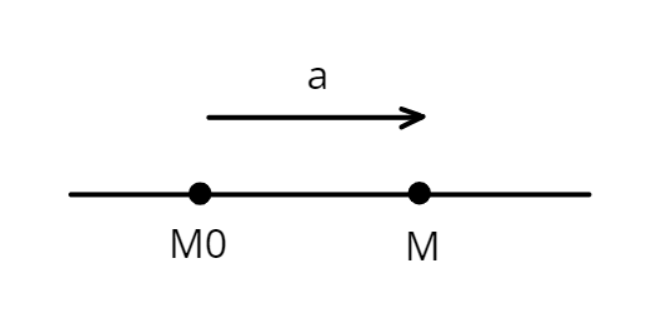
\includegraphics[width=0.4\linewidth]{Прямая в пространстве.PNG}
		\label{fig:mpr}
	\end{figure}\\
	Вектор $\overrightarrow{M_0M}$ имеет координаты $(x - x_0, y - y_0, z - z_0)$. Тогда из $(1)$ мы получим \begin{center}
		$\dfrac{x - x_0}{a_1} = \dfrac{y - y_0}{a_2} = \dfrac{z - z_0}{a_3} = t$ --- \textbf{каноническое уравнение прямой в пространстве.}
	\end{center}
	Отсюда получим 
	\begin{equation*}
		\begin{cases}
			x = x_0 + ta_1, \\
			y = y_0 + ta_2, \\
			z = z_0 + ta_3;
		\end{cases} - \textbf{параметрическое уравнение прямой в пространстве.}
	\end{equation*}\\
	Пусть у нас есть ещё одна точка $M_1(x_1, y_1, z_1)$, которая также принадлежит прямой $\Delta$, тогда в качестве вектора $a$ можно взять вектор $\overrightarrow{M_0M_1}(x_1 - x_0, y_1 - y_0, z_1 - z_0)$. По итогу получаем \begin{center}
		$\dfrac{x - x_0}{x_1 - x_0} = \dfrac{y - y_0}{y_1 - y_0} = \dfrac{z - z_0}{z_1 - z_0}$ --- \textbf{уравнение прямой, проходящей через две точки}.
	\end{center}
	Пусть есть две не параллельные плоскости $\text{П}_1: A_1x + B_1y + C_1z + D_1 = 0$ и $\text{П}_2: A_2x + B_2y + C_2z + D_2 = 0$. Тогда прямую в пространстве можно задать как пересечение этих плоскостей: 
	\begin{equation*}
		\begin{cases}
			\text{П}_1: A_1x + B_1y + C_1z + D_1 = 0 \\
			\text{П}_2: A_2x + B_2y + C_2z + D_2 = 0 
		\end{cases} - \textbf{ уравнение прямой как пересечение двух плоскостей.}
	\end{equation*} 
	\begin{examp}
		 Пусть прямая $\Delta$ задана как пересечение двух плоскостей:
		\begin{equation*}
			\begin{cases}
				\text{П}_1: 2x - 3y + 2z - 5 = 0, \\
				\text{П}_2: 3x + 2y + z - 1 = 0.
			\end{cases} \text{ Задача --- найти параметрическое уравнение этой прямой.}
		\end{equation*} 
		Нужно найти точку, принаждежащую этой прямой, а также направляющий вектор. Точку на прямой будем искать как общую точку для плоскостей, пересечение которых образуют эту прямую. Одну из координат можно взять любой (к примеру, возьмём $z = 0$), тогда получим систему уравнений: 
		\begin{equation*}
			\begin{cases}
				\text{П}_1: 2x - 3y = 5, \\
				\text{П}_2: 3x + 2y = 1; 
			\end{cases}, \text{ решение которого } x = 1, y = -1.
		\end{equation*}
		Тогда искомая точка $A$ имеет координаты $(1, -1, 0)$.\\
		Направляющий вектор можно найти как векторное произведение нормальных векторов плоскостей --- полученный вектор будет параллелен прямой. Для первой плоскости $n_1(2, -3, 2)$, для второй $n_2(3, 2, 1)$. Их векторное произведение: $[n_1, n_2] =$
		$\begin{vmatrix}
			i& j & k \\
			2 & -3 & 2 \\
			3 & 2 & 1
		\end{vmatrix} = -7i + 4j + 13k \Rightarrow a(-7, 4, 13) - \text{направляющий вектор прямой } \Delta$.\\
		В итоге по найдённой точке и направляющему вектору получаем искомое параметрическое уравнение прямой:
		$$\begin{cases}
			x = 1 - 7t, \\
			y = -1 + 4t, \\
			z = 13t.
		\end{cases}$$
	\end{examp}\\
	Рассмотрим взаимное расположение плоскости и прямой в пространстве. Пусть плоскость П задана уравнением $Ax + By + Cz + D = 0 \Rightarrow n(A, B, C)$ --- нормальный вектор плоскости. Прямая же будет иметь направляющий вектор $a(a_1, a_2, a_3) \parallel \Delta$. $M_0(x_0, y_0, z_0) \in \Delta$.
	
	\begin{enumerate}
		\item $\Delta \in \text{П} \Leftrightarrow a \perp n \text{ и } M_0 \in \text{П}$. Последнее возможно $\Leftrightarrow Ax_0 + By_0 + Cz_0 + D = 0$.
		
		\item $\Delta \parallel$ П $\Leftrightarrow a \perp n$ и $M_0 \notin$ П. Последнее возможно $\Leftrightarrow Ax_0 + By_0 + Cz_0 + D \ne 0$.
		
		\item $\Delta$ $\cup$ П $\Leftrightarrow a \not \perp n \Leftrightarrow a \cdot n \ne 0$.
	\end{enumerate}
	Синус угла между прямой и плоскостью можно находить по следующей формуле:
	\begin{center}
		$sin\varphi = \dfrac{n \cdot a}{|n| \cdot |a|} = \dfrac{Aa_1 + Ba_2 + Ca_3}{\sqrt{a_1^2 + a_2^2 + a_3^2}\sqrt{A^2 + B^2 + C^2}}$
	\end{center}
	Рассмотрим взаимное расположение прямых в пространстве. Прямая $\Delta_1$ имеет направляющий вектор $a(a_1, a_2, a_3)$ и точку $M_1(x_1, y_1, z_1)$. Прямая $\Delta_2$ имеет направляющий вектор $b(b_1, b_2, a_3)$ и точку $M_2(x_2, y_2, z_2)$. 
	\begin{enumerate}
		\item Прямые совпадают ($\Delta_1 = \Delta_2$) $\Leftrightarrow$ $a$ $\parallel$ $b$ $\parallel$ $\overrightarrow{M_1M_2}$.
		
		\item Прямые параллельны ($\Delta_1$ $\parallel$ $\Delta_2$) $\Leftrightarrow$ $a$ $\parallel$ $b$ $\nparallel$ $\overrightarrow{M_1M_2}$.
		
		\item Прямые пересекаются ($\Delta_1$ $\cup$ $\Delta_2$) $\Leftrightarrow$ $a$ $\nparallel$ $b$ и $a, b, \overrightarrow{M_1M_2}$ --- компланарные.
		
		\item Прямые не пересекаются и не параллельны ($\Delta_1$ $\dot{-}$ $\Delta_2$) $\Leftrightarrow$ $a$ $\nparallel$ $b$ и $a, b, \overrightarrow{M_1M_2}$ --- некомпланарные.
	\end{enumerate}
	Косинус угла между прямыми можно найти по следующей формуле:
	\begin{center}
		$cos\varphi = \dfrac{a \cdot b}{|a| \cdot |b|}$
	\end{center}
	
	
	
	

\chapter{Линии и поверхности второго порядка}

\section{Эллипс.}

$\bullet$ \textit{\textbf{Эллипс} --- это множество точек плоскости, сумма расстояния от которых до двух данных точек $F_1, F_2$ этой плоскости есть величина постоянная (большая, чем расстояние от $F_1$ до $F_2$). В свою очередь, точки $F_1, F_2$ называются \textbf{фокусами эллипса}.}\\
\begin{wrapfigure}{l}{0.5\textwidth}
	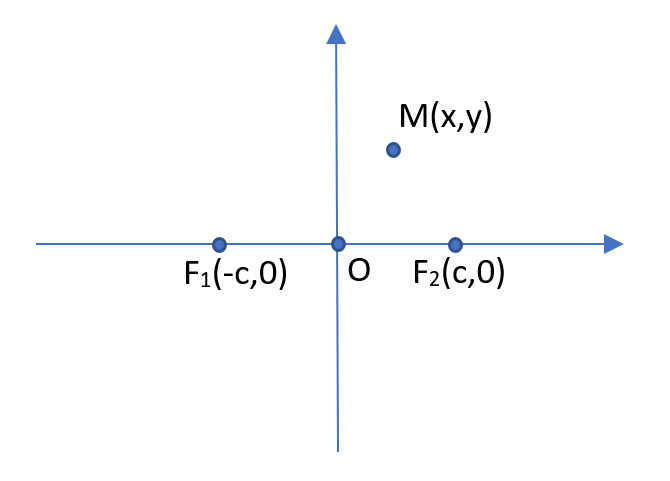
\includegraphics[width=0.5\textwidth]{Эллипс_1.PNG}
	\label{ris:image}
\end{wrapfigure}
Выведем формулу эллипса. Обозначим за $2c$ расстояние между фокусами $F_1(-c, 0)$ и $F_2(c, 0)$. За $2a$ обозначим сумму расстояний от $F_1$ до $M(x, y)$ и от $F_2$ до $M(x, y)$, где $M$ --- точка эллипса. Очевидно, что $2a~>~2c \Rightarrow a > c$. Тогда $2a = \overline{|MF_1|} + \overline{|MF_2|} = \sqrt{(x + c)^2 + y^2} + \sqrt{(x - c)^2 + y^2}$. \\
Второй корень перенесём в правую часть равенства и возведём всё в квадрат. В итоге получим: $x^2 + c^2 + 2xc + y^2 = 4a^2~ -~ 4a\sqrt{(x - c)^2 + y^2} + x^2 + c^2 - 2xc +~ y^2$.\\
Приведём подобные: $4a\sqrt{(x - c)^2 + y^2} = 4a^2 - 4xc$. Поделим на 4 и получим: $a\sqrt{(x - c)^2 + y^2} = a^2 - xc$.\\
Снова обе части возводим в квадрат: $a^2(x^2 + c^2 - 2xc + y^2) = a^4 + x^2c^2 - 2a^2xc$. Раскроем скобки в правой части и приведём подобные: $a^2x^2 + a^2c^2 + a^2y^2 = a^4 + x^2c^2$. Немного преобразуем это равенство: $x^2(a^2 - c^2) + a^2y^2 = a^2(a^2 - c^2)$.\\
Вспомним, что $a > c \Rightarrow a^2 > c^2 \Rightarrow a^2 - c^2 > 0$. Обозначим за $b = \sqrt{a^2 - c^2} \Rightarrow b^2 ~= a^2 - c^2 \Rightarrow$ из равенства получаем: $b^2x^2 + a^2y^2 = b^2a^2$. \\
Поделим обе части на $(a^2b^2)$: \begin{center}$\dfrac{x^2}{a^2} + \dfrac{y^2}{b^2} = 1$ \end{center}\textbf{т.е. любая точка $M(x, y)$, удовлетворяющая этому \underline{каноническому уравнению}, принадлежит эллипсу}.\\\\
Мы показали, что любая точка, удовлетворяющая уравнению $2a = \sqrt{(x + c)^2 + y^2} + \sqrt{(x - c)^2 + y^2}$, удовлетворяет каноническому уравнению. Теперь покажем, что любая точка $M(x_0, y_0)$, удовлетворяющая каноническому уравнению, принадлежит эллипсу (обратная задача).\\
Перепишем каноническое уравнение следующим образом: $\dfrac{y_0^2}{b^2} = 1 - \dfrac{x_0^2}{a^2}$. Домножим на $b^2$ и получим $y_0^2 = b^2(1 - \dfrac{x_0^2}{a^2})$.\\\\
Тогда $\overline{|MF_1|} = \sqrt{(x_0 + c)^2 + y_0^2} = \sqrt{(x_0 + c)^2 + b^2(1 - \dfrac{x_0^2}{a^2})} = \sqrt{x_0^2 + c^2 + 2x_0c + b^2 - b^2\dfrac{x_0^2}{a^2}} = [b^2 = a^2 - c^2] = \sqrt{x_0^2 + c^2 + 2x_0c + a^2 - c^2 - (a^2 - c^2)\dfrac{x_0^2}{a^2}} = \sqrt{2x_0c + a^2 + c^2\dfrac{x_0^2}{a^2}} = \sqrt{(a + \dfrac{cx_0}{a})^2} = |a + \dfrac{cx_0}{a}|$.\\\\
Значит, $\overline{|MF_1|} = |a + \dfrac{c}{a}x_0|$. Аналогично,  $\overline{|MF_2|} = |a - \dfrac{c}{a}x_0|$.\\\\
$\dfrac{x_0^2}{a^2} \leqslant 1 \Leftrightarrow -1 \leqslant \dfrac{x_0}{a} \leqslant 1 \Leftrightarrow -c \leqslant \dfrac{c}{a}x_0 \leqslant c$. Т.к. $c < a \Rightarrow -a \leqslant \dfrac{c}{a}x_0 \leqslant a$.\\\\
Значит, $\overline{|MF_1|} = |a + \dfrac{c}{a}x_0| = a + \dfrac{c}{a}x_0$, $\overline{|MF_2|} = |a - \dfrac{c}{a}x_0| = a - \dfrac{c}{a}x_0$.\\\\
$\overline{|MF_1|} + \overline{|MF_2|} = a + \dfrac{c}{a}x_0 + a - \dfrac{c}{a}x_0 = 2a \Rightarrow \forall$ точка, удовлетворяющая каноническому уравнению, принадлежит эллипсу.
\\\\\
Исследуем форму эллипса.\\
\begin{wrapfigure}{l}{0.5\textwidth}
	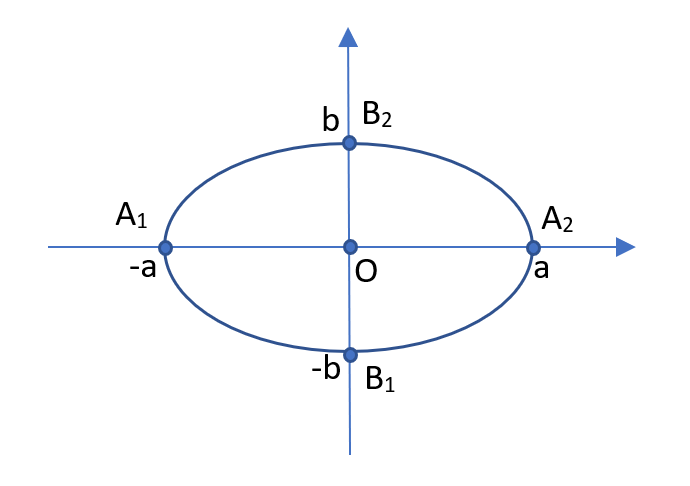
\includegraphics[width=0.5\textwidth]{Эллипс_2.PNG}
	\label{ris:image}
\end{wrapfigure}
Рассмотрим каноническое уравнение эллипса $\dfrac{x^2}{a^2} + \dfrac{y^2}{b^2} = 1$. Из него следует, что $\dfrac{x^2}{a^2} \leqslant 1 \Rightarrow |x| \leqslant a$. Аналогично $\dfrac{y^2}{b^2} \leqslant 1 \Rightarrow |y| \leqslant b$. Значит, эллипс ограничен прямоугольником, а его вершины имеют координаты $A_1(-a, 0), A_2(a, 0), B_1(0, -b), B_2(0, b)$. 

Если точка $M_1(x, y)$ принадлежит эллипсу, то и точки $M_2(-x, y), M_3(x, -y), M_4(-x, -y)$ принаждлежат эллипсу $\Rightarrow$ эллипс симметричек относительно осей $O_x$ и $O_y$, а точка $O$ --- \textbf{центр эллипса}.\\
Прямая, проходящая через фокусы --- \textbf{большая ось эллипса}, а перпендикулярная --- \textbf{малая ось эллипса}. $a, b$ --- полуоси.\\\\
Рассмотрим 1-ю четверть, где $x \geq 0$ и $y \geq 0$. Выразим из уравнения $y$: $y^2 = b^2(1 - \dfrac{x^2}{a^2}) \Rightarrow y = b\sqrt{1 - \dfrac{x^2}{a^2}} \Rightarrow y = \dfrac{b}{a}\sqrt{a^2 - x^2}$.\\\\
Возьмём производную: $y' = \dfrac{-2bx}{2a\sqrt{a^2 - x^2}} = -\dfrac{b}{a}\dfrac{x}{\sqrt{a^2 - x^2}} < 0 \Rightarrow y$ убывает.\\\\
Возьмём вторую производную: $y'' = -\dfrac{b}{a}(\dfrac{1}{\sqrt{a^2 - x^2}} + 2x(-1)\dfrac{1}{2}\dfrac{1}{\sqrt{a^2-x^2}^3}) = -\dfrac{b}{a}\dfrac{a^2 - x^2 + x^2}{\sqrt{a^2-x^2}^3} = \dfrac{-ba}{\sqrt{a^2-x^2}^3} < 0 \Rightarrow$ функция выпукла вверх. Аналогично можно рассмотреть эллипс в других четвертях.\\
\begin{examp}
$\dfrac{x^2}{25} + \dfrac{y^2}{9} = 1$. \\\\
$a^2 = 25 \Rightarrow a = 5, b^2 = 9 \Rightarrow b = 3$.
\begin{center}  
	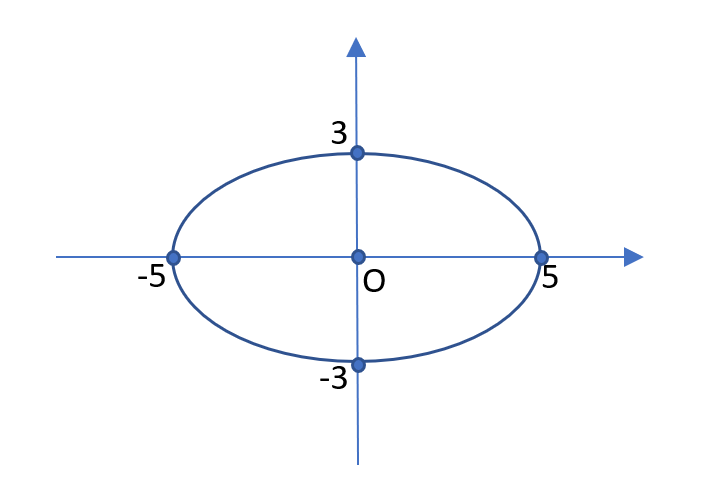
\includegraphics[width=0.5\textwidth]{Эллипс_3.PNG}
\end{center}
\end{examp}





\section{Гипербола.}

\begin{wrapfigure}{l}{0.5\textwidth}
	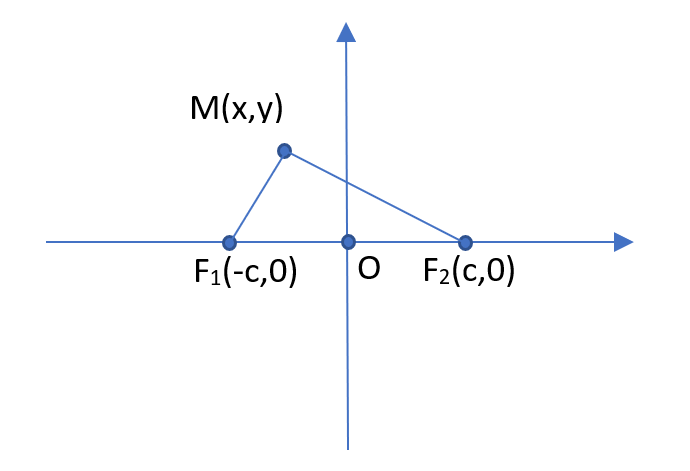
\includegraphics[width=0.5\textwidth]{Гипербола_1.PNG}
	\label{ris:image}
\end{wrapfigure}
$\bullet$ \textit{\textbf{Гипербола} --- это множество всех точек плоскости, модуль разности расстояний от которых до двух данных точек $F_1$ и $F_2$ (\textbf{фокусы}) есть величина постоянная и меньше, чем $\overline{|F_1F_2|}$}.\\\\
Рассмотрим упомянутые расстояния: $\overline{|MF_1|} = \sqrt{(x+c)^2 + y^2}; \overline{|MF_2|} = \sqrt{(x-c)^2 + y^2}$. $|\overline{|MF_1|} - \overline{|MF_2|}| = 2a < 2c \Rightarrow ~a ~< ~c$.\\\\
$|\sqrt{(x+c)^2 + y^2} - \sqrt{(x-c)^2 + y^2}| = 2a$ --- \textbf{уравнение гиперболы}.\\\\
Преобразуем данное уравнение. Раскроем модуль и перенесём второй корень в правую часть: $\sqrt{(x+c)^2 + y^2} = \sqrt{(x-c)^2 + y^2} \pm 2a$. Возведём обе части в квадрат: $(x+c)^2 + y^2 = (x-c)^2 + y^2 + 4a^2 \pm 4a\sqrt{(x-c)^2 + y^2}$.\\
Расскрывая скобки и приведя подобные, получим $4xc = 4a^2 \pm 4a\sqrt{(x-c)^2 + y^2}$. Обе части можно поделить на 4: $xc = a^2 \pm a\sqrt{(x-c)^2 + y^2}$.\\
Перенесём $a^2$ вправо и возведём ещё раз в квадрат: $x^2c^2 + a^4 + 2a^2xc = a^2x^2 + a^2c^2 - 2a^2xc + a^2y^2$. Приведя подобные и вынеся общие члены за скобки, получим $x^2(c^2 - a^2) - a^2y^2 = a^2(c^2 - a^2)$.\\
Обозначим за $b = \sqrt{c^2 - a^2}$ и сделаем замену: $x^2b^2 - a^2y^2 = a^2b^2$. Поделим всё на $a^2b^2$ и получим \textbf{каноническое уравнение гиперболы}: $$\dfrac{x^2}{a^2} - \dfrac{y^2}{b^2} = 1.$$
Теперь покажем, что любая точка $M(x, y)$, удовлетворяющая каноническому уравнению, принадлежит гиперболе.\\
Из канонического уравнения $y^2 = (\dfrac{x^2}{a^2} - 1)b^2$. $\overline{|MF_1|} = \sqrt{(x+c)^2 + y^2} = \sqrt{x^2+c^2+2xc+b^2\dfrac{x^2}{a^2}-b^2} = \sqrt{x^2 + c^2 + 2xc+ c^2\dfrac{x^2}{a^2} - x^2 - c^2 + a^2} = \sqrt{a^2 + (\dfrac{cx}{a})^2 + 2xc} = |a + \dfrac{c}{a}x|$. Аналогичным образом $\overline{|MF_2|} = |a - \dfrac{c}{a}x|$.\\\\
Т.к. $\dfrac{x^2}{a^2} \leqslant 1 \Rightarrow x^2 \delta a^2 \Rightarrow $ имеем два случая\begin{enumerate}
	\item $x \leqslant a \Rightarrow \dfrac{x}{a} \leqslant 1 \Rightarrow \dfrac{c}{a}x \geqslant c$. Но $c > a \Rightarrow \overline{|MF_1|} = a + \dfrac{c}{a}x, \overline{MF_2} = \dfrac{c}{a}x - a$ и $\big|\overline{|MF_1|} - \overline{|MF_2|}\big| = |a + \dfrac{c}{a}x - \dfrac{c}{a}x - a| = 2a$.
	\item $x \leq -a \Rightarrow -\dfrac{x}{a} \leqslant 1 \Rightarrow -\dfrac{c}{a}x \leqslant c > a \Rightarrow \overline{|MF_1|} = -a - \dfrac{c}{a}x, \overline{MF_2} = a - \dfrac{c}{a}x$ и $\big|\overline{|MF_1|} - \overline{|MF_2|}\big| = |-a - \dfrac{c}{a}x - a + \dfrac{c}{a}x| = 2a$.
\end{enumerate}
Исследуем форму гиперболы.\\
Пересечения: точки $A_1(-a, 0) и A_2(a, 0)$ --- с осью $O_x$, а с осью $O_y$ пересечений нет.\\
Гипербола симметрична относительно $O_x$ и $O_y$ (из-за квадратов в каноническом уравнении). Ось $O_x$ --- \textbf{действительная ось гиперболы} (на ней лежат точки $F_1, F_2$), ось $O_y$ --- \textbf{мнимая ось гиперболы}.\\
Середина $\overline{F_1F_2}$ --- \textbf{центр гиперболы}. Точки $A_1, A_2$ --- \textbf{вершины гиперболы}, $a, b$ --- \textbf{полюсы гиперболы}. Если $a = b$, то гиперболу называют \textbf{равносторонней}.\\\\
Рассмотрим гиперболу в первой четверти. $y^2 = (\dfrac{x^2}{a^2} - 1)b^2 \Rightarrow y^2 = \dfrac{b^2}{a^2}(x^2-a^2) \Rightarrow y = \dfrac{b}{a}\sqrt{x^2-a^2}$.\\\\
$y' = \dfrac{b}{a}\cdot\dfrac{1}{2}\cdot\dfrac{2x}{\sqrt{x^2-a^2}}=\dfrac{bx}{a\sqrt{x^2-a^2}} > 0 \Rightarrow y$ возрастает.\\\\
$y'' = \dfrac{b}{a}\cdot\Big(\dfrac{\sqrt{x^2-a^2} - x - \dfrac{2x}{\frac{2}{\sqrt{x^2 - a^2}}}}{x^2 - a^2}\Big) = \dfrac{b}{a}\cdot\Big(\dfrac{x^2 - a^2 - x^2}{(x-a)^2\sqrt{x^2-a^2}}\Big) = \dfrac{-ab}{(\sqrt{x^2-a^2})^3} < 0 \Rightarrow$ функция выпукла вверх по $y$.\\
\begin{figure}[h]
	\centering
	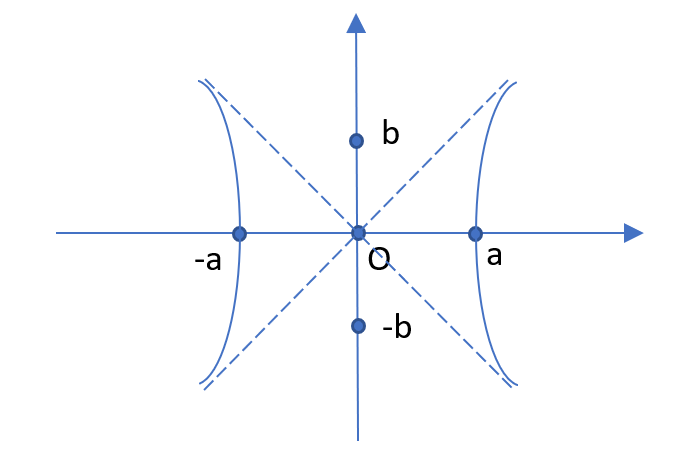
\includegraphics[width=0.5\textwidth]{Гипербола_2.PNG}
	\label{fig:mpr}
\end{figure}\\
Асимптоты гиперболы должны удовлетворять формуле $y = kx + l$. $k = \lim\limits_{x \to +\infty}\dfrac{f(x)}{x} = \lim\limits_{x \to +\infty}\dfrac{b\sqrt{x^2 - a^2}}{x} = \dfrac{b}{a}$. \\\\
$l = \lim\limits_{x \to +\infty} f(x) - kx = \lim\limits_{x \to +\infty}\Big(\dfrac{b}{a}\sqrt{x^2-a^2} - \dfrac{b}{a}x = \dfrac{b}{a}\lim\limits_{x \to +\infty}\dfrac{-a^2}{\sqrt{x^2-a^2}+x}\Big) = 0 \Rightarrow$ 
асимптоты: $y = \dfrac{b}{a}x; y = -\Big(\dfrac{b}{a}x\Big)$.\\
\begin{figure}[h]
	\centering
	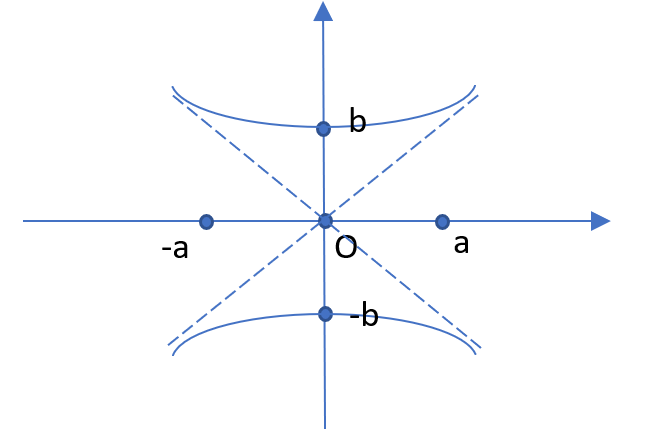
\includegraphics[width=0.5\textwidth]{Гипербола_3.PNG}
	\label{fig:mpr}
\end{figure}\\
Сопряженная гипербола. Её точки удовлетворяют каноническому уравнению $\dfrac{y^2}{b^2} - \dfrac{x^2}{a^2} = 1$.\\
\begin{examp}
	$\dfrac{x^2}{25} - \dfrac{y^2}{9} = 1.\\ a = 5, b = 3$. Асимптоты удовлетворяю уравнению $y = \pm\dfrac{3}{5}x$. 
	\begin{center}  
		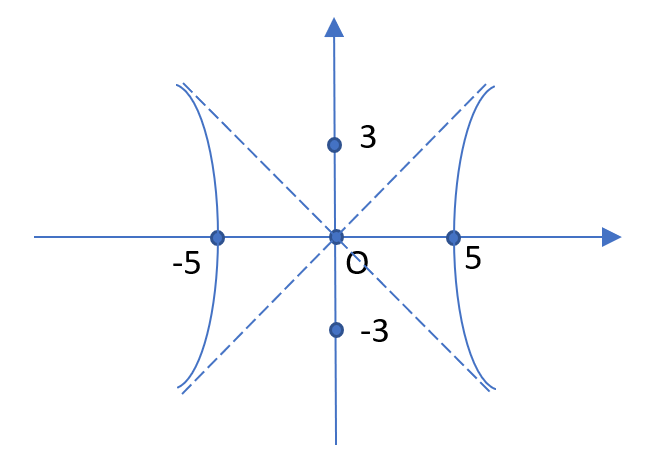
\includegraphics[width=0.5\textwidth]{Гипербола_4.PNG}
	\end{center}
\end{examp}





\section{Эксцентриситет и директрисы эллипса и гиперболы.}

Вспомним формулы их двух прошлых параграфов:\\
$2c$ --- растояние между фокусами.\\
Эллипс: $\dfrac{x^2}{a^2} + \dfrac{y^2}{b^2} = 1$, $a > c, b = a^2 - c^2$.\\
Гипербола: $\dfrac{x^2}{a^2} - \dfrac{y^2}{b^2} = 1$, $c > a, b = c^2 - a^2$.\\\\
$\bullet$ \textit{\textbf{Эксцентриситет} --- величина, равная $\varepsilon = \dfrac{c}{a}$}.\\\\
\textbf{Утверждение:} \textit{для эллипса $c < a \Rightarrow 0 < \varepsilon < 1$}: $\varepsilon = \dfrac{c}{a} = \dfrac{\sqrt{a^2 - b^2}}{a} = \sqrt{1 - \Big(\dfrac{b}{a}\Big)^2}$. \textit{Для гиперболы} $c > a \Rightarrow \varepsilon > 1$: $\varepsilon = \dfrac{c}{a} = \dfrac{\sqrt{a^2+b^2}}{a} = \sqrt{1 + \Big(\dfrac{b}{a}\Big)^2}$.\\ Чем больше эксцентриситет, тем уже эллипс (гипербола).
\begin{center}
	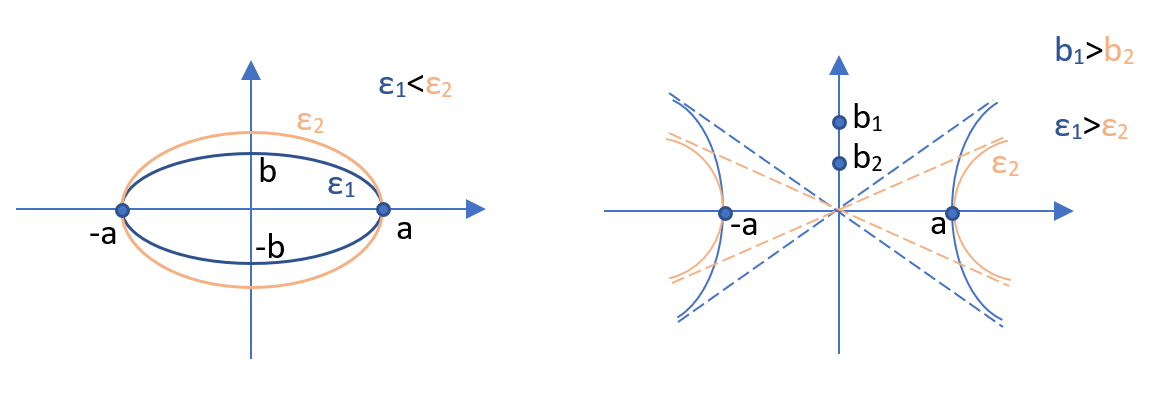
\includegraphics[width=1\textwidth]{Эксцентриситет_1.PNG}
\end{center}
$\bullet$ \textit{\textbf{Директрисы} --- прямые, проходящие параллельно малой оси эллипса (мномой оси гиперболы) на расстоянии $\dfrac{a}{\varepsilon}$ от центра эллипса (гиперболы)}.
\begin{center}
	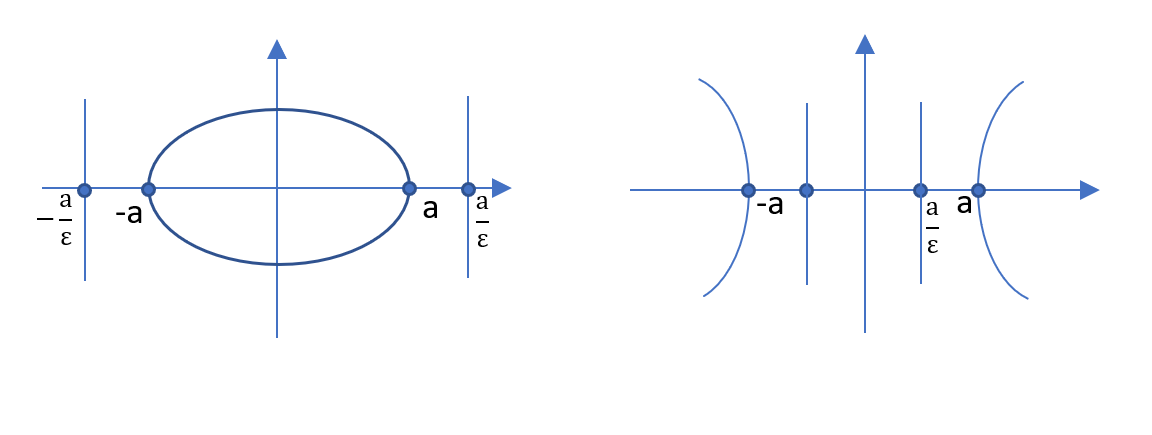
\includegraphics[width=1\textwidth]{Эксцентриситет_2.PNG}
\end{center}
$\bullet$ \textit{Директриса и фокус, расположенные по одну сторону от $O_y$, называются \textbf{соответствующими}}.\\\\
$\rho(F_i, \Delta_i) = |c - \dfrac{a}{\varepsilon}|, i = \overline{1, 2}; F_1(-c, 0), F_2(c, 0)$.
\newtheorem*{th18}{Теорема (основное свойство директрис)}\begin{th18}Пусть $M(x, y)$ --- любая точка эллипса/гиперболы. Тогда $\varepsilon = \dfrac{\overline{|MF_i|}}{\rho(M, \Delta_i)}$, где $\Delta_i, F_i$ --- соответствующие.
\end{th18}
\begin{Proof}
	Докажем для эллипса. Для гиперболы доказательство аналогичное. Достаточно рассмотреть оба случая ($i = 1$ и $i = 2$):\\\\
	$\dfrac{\overline{|MF_2|}}{M, \Delta_2)} = \dfrac{a - \varepsilon_x}{\dfrac{a}{\varepsilon} - x} = \varepsilon$.\\\\
	$\dfrac{\overline{|MF_1|}}{M, \Delta_1)} = \dfrac{a + \varepsilon_x}{\dfrac{a}{\varepsilon} + x} = \varepsilon$.
\end{Proof}




\section{Парабола.}

Пусть $F$ --- точка на плоскости (фокус). $F \notin \Delta$, где $\Delta$ --- директриса.\\
\begin{wrapfigure}{l}{0.5\textwidth}
	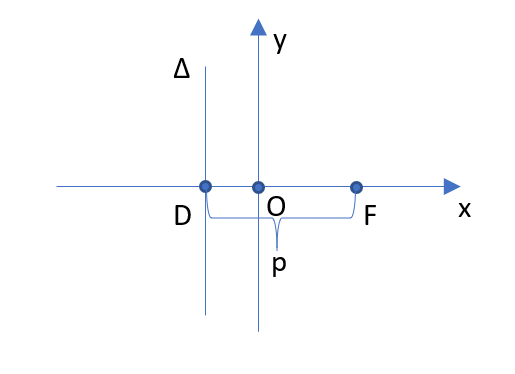
\includegraphics[width=0.5\textwidth]{Парабола_1.PNG}
	\label{ris:image}
\end{wrapfigure}
$\bullet$ \textit{\textbf{Парабола} --- множество точек плоскости, каждая из которых равноудалена от $F$ и от $\Delta$}.\\\\
Введём обозначения. $p = \overline{|DF|}, F(\dfrac{p}{2}, 0), \Delta: x = -\dfrac{p}{2}, M(x, y)$ --- точка, принадлежащая параболе, $\rho(M, \Delta) = \overline{|MF|}$.\\\\
$|x + \dfrac{p}{2}| = \sqrt{(x - \dfrac{p}{2})^2+y^2}$ из определения параболы. Возведём обе части в квадрат: $x^2 + px + \dfrac{p^2}{4} = x^2 - px + \dfrac{p^2}{4} + y^2 \Rightarrow$ \begin{center}
	$y^2 = 2px$ --- \textbf{каноническое уравнение параболы}.
\end{center}
Покажем, что любая точка $M_1(x_1, y_1)$, удовлетворяющая каноническому уравнению, принадлежит эллипсу.\\ $\overline{|M_1F|} = \sqrt{(x_1 - \dfrac{p}{2})^2 + y_1^2} = \sqrt{x_1^2 + \dfrac{p^2}{4} - 2px_1 - px_1} = \sqrt{x_1^2 + \dfrac{p^2}{4} + px_1} = \sqrt{(x_1 + \dfrac{p}{2})^2} = |x_1 + \dfrac{p}{2}| = \rho(M_1, \Delta) \Rightarrow \overline{|M_1F|} = \rho(M_1, \Delta)$.
\newtheorem*{cor19}{Следствие}\begin{cor19}
	\begin{enumerate}
		\item  $x \geqslant 0$ --- парабола в \underline{правой} полуплоскости;
		\item Если точка $M(x, y) \in$ параболе, то и $M'(x, -y) \in$ параболе;
		\item Ось, проходящая через фокусы --- \textbf{ось симметрии};
		\item $y \geqslant 0: y = \sqrt{px} \Rightarrow y' = \dfrac{\sqrt{2p}}{2\sqrt{x}} > 0 \Rightarrow y$ возрастает.
	\end{enumerate}
\end{cor19}
\begin{center}
	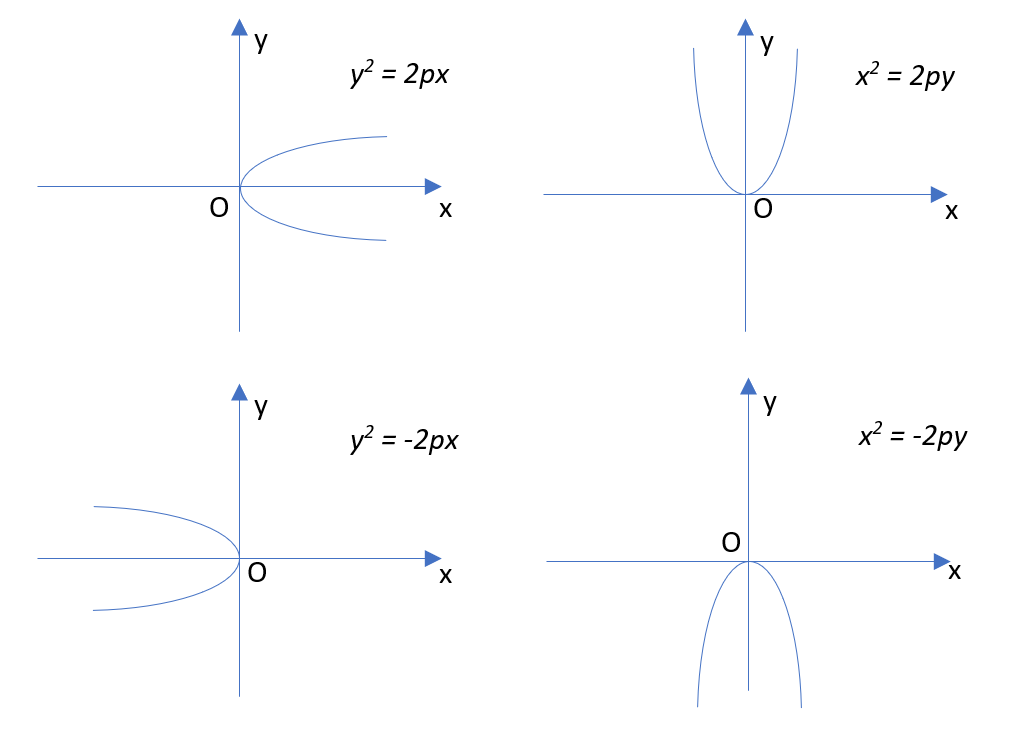
\includegraphics[width=0.65\textwidth]{Парабола_2.PNG}
\end{center}






\section{Линии второго порядка.}

$\bullet$ \textit{\textbf{Линии второго порядка} --- это множество точек плоскости, координаты которых удовлетворяют следующему уравнению: $Ax^2 + 2Bxy + Cy^2 + 2Dx + 2Ey + F = 0$, где A, B, C не обращаются одновременно в нуль $(A^2 + B^2 + C^2 \neq 0)$.}\\
\begin{wrapfigure}{l}{0.5\textwidth}
	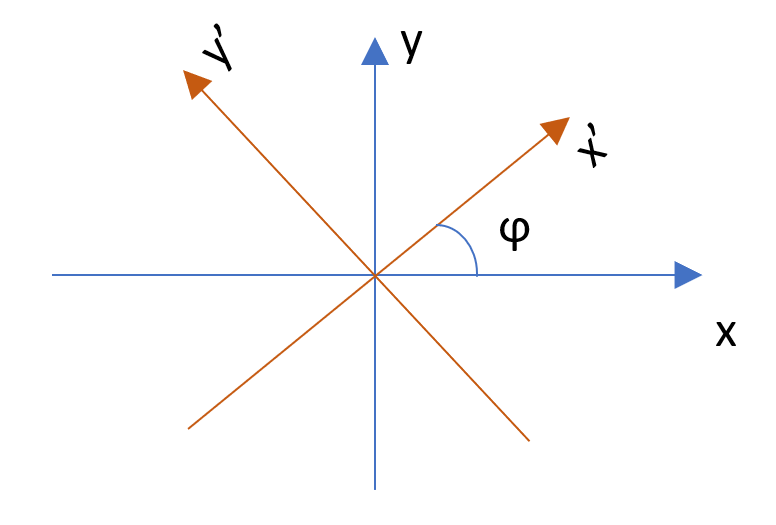
\includegraphics[width=0.5\textwidth]{Л2П_1.PNG}
	\label{ris:image}
\end{wrapfigure}
Выведем некоторые линии второго порядка. Пусть $B \neq 0$ в $O{xy}$. Преобразуем ДПСК $O{xy}$ в $O'{x'y'}$ поворотом на угол $\varphi$. Тогда
$$ \begin{cases}
	x = x' cos\varphi - y' sin\varphi,\\
	y = x' sin\varphi + y' cos\varphi.
\end{cases}
$$
Подставив всё в уравнение для линий второго порядка, получим\\
$A(x'cos\varphi - y'sin\varphi)^2 + 2B(x' cos\varphi - y' sin\varphi)(x' sin\varphi + y' cos\varphi) + C(x' sin\varphi + y' cos\varphi)^2 + 2D(x' cos\varphi - y' sin\varphi) + 2E(x' sin\varphi + y' cos\varphi) + F = 0$.\\
Расскроем скобки и сделаем следующие замены:\\\\
$\begin{cases}
	A' = Acos^2\varphi + 2Bcos\varphi sin\varphi + Csin^2\varphi \\
	B' = -Acos\varphi sin\varphi + B(cos^2\varphi - sin^2\varphi) + Csin\varphi cos\varphi\\
	C' = Asin^2\varphi - 2Bsin\varphi cos\varphi + Ccos^2\varphi \\
	D' = D(x' cos\varphi - y' sin\varphi) \\
	E' = E(x' sin\varphi + y' cos\varphi) \\
	F' = F
\end{cases}$\\
В итоге получим $A'x'^2 + 2Bx'y' + C'y'^2 + 2D'x' + 2E'y' + F' = 0$.\\
Покажем, что $A', B'$ и $C'$ не обращаются в нуль одновременно от противного: пусть $A' = B' = C' = 0$. Тогда, рассмотрев первые три равенства в замене, сложим 1 и 3 уравнение и получим систему:\\
$\begin{cases}
	Acos2\varphi + Bsin2\varphi = 0 \\
	-Asin2\varphi + Bcos2\varphi = 0
\end{cases}$\\
Найдём определитель методом крамера:\\
$\Delta = \begin{vmatrix}
	cos2\varphi & sin2\varphi \\
	-sin2\varphi & cos2\varphi
\end{vmatrix} = cos^22\varphi + sin^22\varphi = 1$;\\
$\Delta_1 =  \begin{vmatrix}
	0 & sin2\varphi \\
	0 & cos2\varphi
\end{vmatrix} = 0$;\\
$\Delta_2 =  \begin{vmatrix}
	cos2\varphi & 0 \\
	-sin2\varphi & 0
\end{vmatrix} = 0$.\\
Значит $A = \dfrac{\Delta_1}{\Delta} = 0, B = \dfrac{\Delta_2}{\Delta} = 0$.\\
Т.к. $B' = 0$, то $B(cos^2\varphi - sin^2\varphi) + (C - A)cos\varphi sin\varphi = 0 \Leftrightarrow Bcos2\varphi + \dfrac{C - A}{2}sin2\varphi = 0$. От сюда получаем, что $tg2\varphi = \dfrac{2B}{A - C}$ --- угол, на который нужно повернуть оси.\\
Если $A = C$, то $\varphi = \dfrac{\pi}{4}$. При повороте на этот угол получаем новую систему координат.\\
Рассмотрим следующие случаи:\begin{enumerate}
	\item $A'C' \neq 0$.\\
	$A'\Big((x')^2 + \dfrac{2D'}{A'}x' + (\dfrac{D'}{A'})^2\Big) - \dfrac{D'^2}{A'} + C'\Big((y')^2 + 2\dfrac{E'}{C'}y' + (\dfrac{E'}{C'})^2\Big) - \dfrac{E'^2}{C'} + F = 0$.\\\\
	Преобразуем, чтобы получить квадраты сумм:\\\\
	$A'\Big(x' + \dfrac{D'}{A'}\Big)^2 + C'\Big(y' + \dfrac{E'}{C'}\Big)^2 + F - \dfrac{(D')^2}{A'} - \dfrac{(E')^2}{C'} = 0$. \\\\
	Сделаем замену: $\begin{cases}
		F' = F - \frac{(D')^2}{A'} - \frac{(E')^2}{C'}, \\
		x'' = x' + \frac{D'}{A'}, \\
		y'' = y' + \frac{E'}{C'};
	\end{cases}$ --- параметрический сдвиг координатных~ осей.\\\\
	Получим $A'(x'')^2 + C'(y'')^2 + F' = 0 \Leftrightarrow \dfrac{(x'')^2}{-\frac{F'}{A'}} + \dfrac{(y'')^2}{-\frac{F'}{C'}} = 1$.\\\\
	Если $-\dfrac{F'}{A'} > 0, -\dfrac{F'}{C'} > 0$, то заменив соответствующие дроби на $a^2, b^2$ получим $\dfrac{(x'')^2}{a^2} + \dfrac{(y'')^2}{b^2} = 1$ --- эллипс.\\\\
	Если $-\dfrac{F'}{A'} < 0, -\dfrac{F'}{C'} < 0$, то получим $\dfrac{(x'')^2}{a^2} + \dfrac{(y'')^2}{b^2} = -1$ --- мнимый эллипс.\\\
	Если же эти дроби разных знаков, то получим $\dfrac{(x'')^2}{a^2} - \dfrac{(y'')^2}{b^2} = 1$ --- гипербола.\\\\
	В итоге получили несколько линий 2-го порядка:
	
	1. $\dfrac{x^2}{a^2} + \dfrac{y^2}{b^2} = 1$ --- эллипс;
	
	2. $\dfrac{x^2}{a^2} + \dfrac{y^2}{b^2} = -1$ --- мнимый эллипс;
	
	3. $\dfrac{x^2}{a^2} - \dfrac{y^2}{b^2} = 1$ --- гипербола;
	
	4. $\dfrac{x^2}{a^2} + \dfrac{y^2}{b^2} = 0$ --- пара мнимых пересекающихся прямых (точка);
	
	5. $\dfrac{x^2}{a^2} - \dfrac{y^2}{b^2} = 0$ --- пара пересекающихся прямых (точка);
	
	Уравнение для прямых и мнимых прямых можно получить при условии, если $F' = 0$. Тогда $A'(x'')^2 + C'(y'')^2 = 0 \Rightarrow \dfrac{x^2}{a^2} + \dfrac{y^2}{b^2} = 0$.
	\item  $A'C' = 0 \Rightarrow A' \neq 0, C = 0$.\\
	$A'(x')^2 + 2D'x' + 2E'y' + F = 0.\ A' \neq 0$.
	
	$A'\Big((x')^2 + \dfrac{2D'}{A'}x' + (\dfrac{D'}{A'})^2\Big) - \dfrac{(D')^2}{A'} + 2E'y' + F = 0$.
	
	Рассмотрим случай, когда $E' \neq 0$. Тогда $A'(x' + \dfrac{D'}{A'})^2 + 2E'(y' + \dfrac{F}{2E'} - \dfrac{(D')^2}{2E'A'}) = 0$. Сделав замену $x'' = x' + \dfrac{D'}{A'},\ y'' = y' + \dfrac{F}{2E'} - \dfrac{(D')^2}{2E'A'}$ получим $A'(x'')^2 + 2E'y'' = 0 \Rightarrow (x'')^2 = -\dfrac{2E'}{A'}y'' \Rightarrow [-\dfrac{2E'}{A'} = 2p] \Rightarrow (x'')^2 = 2py''$ --- уравнение параболы.
	
	Случай, когда $E' = 0$. Тогда $A'(x' + \dfrac{D'}{A'})^2 + F - \dfrac{D'^2}{A} = 0$. Заменим $F' = F - \dfrac{D'^2}{A}, x'' = x' + \dfrac{D'}{A'}, y'' = y' \Rightarrow A'x''^2 + F' = 0 \Rightarrow x''^2 = -\dfrac{F'}{A'}$.
	
	Если $-\dfrac{F'}{A'} > 0$, то $(x'')^2 = a^2 \Rightarrow x'' = \pm a$.
	
	Если $-\dfrac{F'}{A'} < 0$, то $(x'')^2 = -a^2$. Если $-\dfrac{F'}{A'} \Rightarrow (x'')^2 = 0$.
	
	В итоге получили:
	
	6. $y^2 = 2px$ --- парабола;
	
	7. $x^2 - a^2 = 0$ --- пара параллельных прямых;
	
	8. $x^2 + a^2 = 0$ --- пара мнимых параллельных прямых;
	
	9. $x^2 = 0$ --- пара пересекающихся прямых.
\end{enumerate}
\newtheorem*{th20}{Теорема}\begin{th20}
	Для любой линии второго порядка существует система координат, в которой эта линия определена одним из следующих канонических уравнений:
	
	1. $\dfrac{x^2}{a^2} + \dfrac{y^2}{b^2} = 1$ --- эллипс;
	
	2. $\dfrac{x^2}{a^2} + \dfrac{y^2}{b^2} = -1$ --- мнимый эллипс;
	
	3. $\dfrac{x^2}{a^2} - \dfrac{y^2}{b^2} = 1$ --- гипербола;
	
	4. $\dfrac{x^2}{a^2} + \dfrac{y^2}{b^2} = 0$ --- пара мнимых пересекающихся прямых (точка);
	
	5. $\dfrac{x^2}{a^2} - \dfrac{y^2}{b^2} = 0$ --- пара пересекающихся прямых (точка);
	
	6. $y^2 = 2px$ --- парабола;
	
	7. $x^2 - a^2 = 0$ --- пара параллельных прямых;
	
	8. $x^2 + a^2 = 0$ --- пара мнимых параллельных прямых;
	
	9. $x^2 = 0$ --- пара пересекающихся прямых.
\end{th20}
\begin{examp}
	Определить, какая линия второго порядка задана уравнением и нарисовать её на плоскости:
	$x^2 - 12xy - 4y^2 + 12x + 8y + 5 = 0$.\\
	$A = 1, C = -4, 2B = -12$.\\
	Найдём угол $\varphi$, на который нужно повернуть ДПСК:\\
	$tg2\varphi = \dfrac{2B}{A - C} = -\dfrac{12}{5}$. Из тригонометрии: $tg2\varphi = \dfrac{2tg\varphi}{1 - tg^2\varphi}$. Заменим $tg\varphi = t$.\\
	$\dfrac{2t}{1-t^2} = -\dfrac{12}{5} \Rightarrow \dfrac{t}{1-t^2} = -\dfrac{6}{5}$.
	\\
	$6t^2 - 5t - 6 = 0 \Rightarrow t = \dfrac{5 + 13}{12} = \dfrac{3}{2} \Rightarrow tg\varphi \dfrac{3}{2}$.
	\\
	От сюда:
	$sin\varphi = \dfrac{3}{\sqrt{13}}, cos\varphi = \dfrac{2}{\sqrt{13}}$
	\\
	Делаем замену, переходя к новой ДПСК:
	\\
	$\begin{cases}
		x = \dfrac{1}{\sqrt{13}}(2x'-3y') \\
		y = \dfrac{1}{\sqrt{13}}(3x' + 2y')
	\end{cases}$
	\\
	Подставляем:
	\\
	$\dfrac{1}{13}(4x'^2 - 12x'y' + 9y'^2) - \dfrac{12}{13}(6x'^2 - 6y'^2 - 5x'y') - \dfrac{4}{13}(9x'^2 + 12x'y' + 4y'^2) + \dfrac{12}{\sqrt{13}}(2x'-3y') + \dfrac{8}{\sqrt{13}}(3x'+2y') + 5 = 0$
	\\
	Задача была получить 0 перед $x'y'$. Проверим, найдя коэффициенты перед множителями:
	\\
	$x'^2: \dfrac{4}{13} - \dfrac{72}{13} - \dfrac{36}{13} = -8$
	\\
	$y'^2: \dfrac{9}{13} + \dfrac{72}{13} - \dfrac{16}{13} = 5$
	\\
	$x'y': -\dfrac{12}{13} + \dfrac{60}{13} - \dfrac{48}{13} = 0$
	\\
	В итоге получили: $-8x'^2 + 5y'^2 + \dfrac{48}{\sqrt{13}}x' - \dfrac{20}{\sqrt{13}}x' - \dfrac{20}{\sqrt{13}}y' + 5 = 0$.
	\\
	Теперь сделаем ещё одно преобразование ДПСК: параллельный перенос (таким образом, мы избавимся от $x'$ и $y'$, оставив только $x'^2$ и $y'^2$).
	\\
	Преобразуем: $-8(x'^2 - \dfrac{6}{\sqrt{13}}x' + \dfrac{9}{13}) + \dfrac{72}{13} + 5(y'^2 - \dfrac{4}{\sqrt{13}}y' + \dfrac{4}{13}) - \dfrac{20}{13} + 5 = 0 \Leftrightarrow -8(x' - \dfrac{3}{\sqrt{13}})^2 + 5(y' - \dfrac{2}{\sqrt{13}})^2 + 9 = 0$
	\\
	Делаем замену, переходя к новой ДПСК:
	\\
	$\begin{cases}
		x'' = x' - \dfrac{3}{\sqrt{13}} \\
		y'' = y' - \dfrac{2}{\sqrt{13}}
	\end{cases}$
	\\
	Подставляем:
	\\
	$-8x''^2 + 5y''^2 + 9 = 0 \Leftrightarrow \dfrac{x''^2}{\dfrac{9}{8}} - \dfrac{y''^2}{\dfrac{9}{5}} = 1$ --- гипербола.
	\\
	$a^2 = \dfrac{9}{8}, b^2 = \dfrac{9}{5}$
	\\
	Некоторые точки искомой линии второго порядка: $(2, 3), (-3, 2)$.
	\\
	На рисунке преобразованные ДПСК отмечены так: синия --- изначальная, оранжевая --- после поворота, зелённая --- после параллельного переноса. Сама линия 2-го порядка (гипербола) нарисована фиолетовым. Иллюстрация примерная (более точный график был сделал в десмосе ниже).
	\begin{center}
		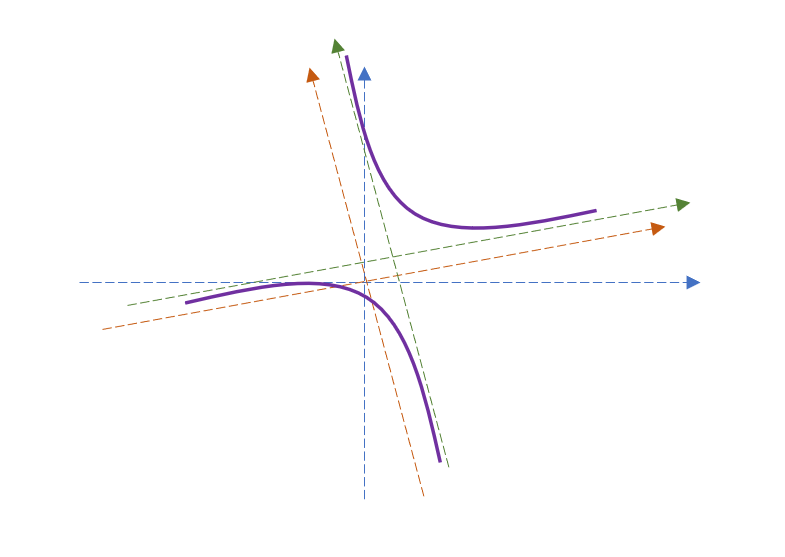
\includegraphics[scale=0.8]{Л2П_2.PNG}
	\end{center}
	\begin{center}
		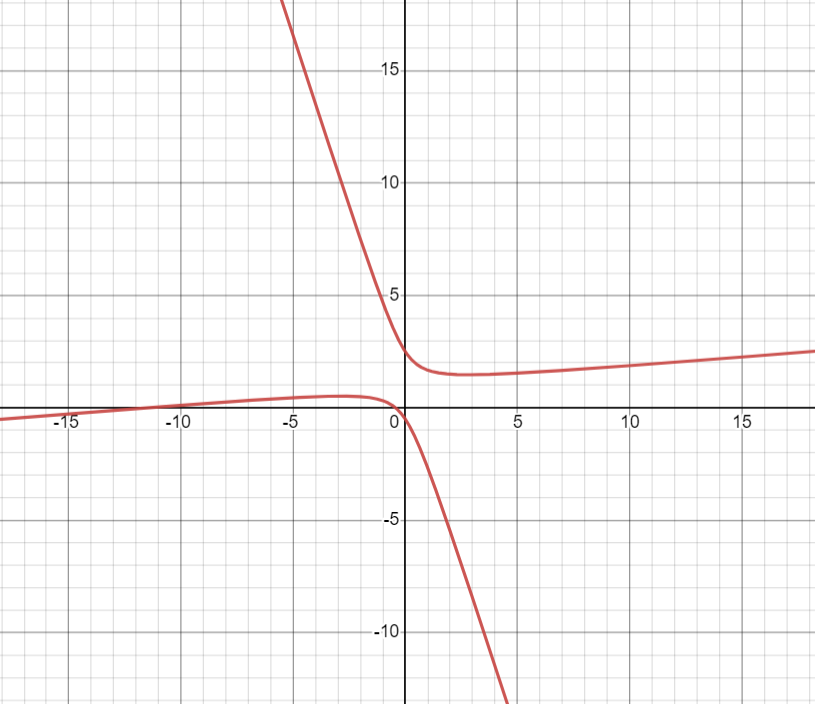
\includegraphics[scale=0.8]{Л2П_3.PNG}
	\end{center}
\end{examp}






\section{Поверхности второго порядка.}

$\bullet$ \textit{\textbf{Поверхность второго порядка} --- множество точек пространства, координаты которых удовлетворяют уравнению следующего вида: $a_{11}x^2 + a_{22}y^2 + a_{33}z^2 + 2a_{12}xy + 2a_{13}xz + 2a{23}_yz + 2a_1x + 2a_2y _ 2a_3z + a = 0$}.
\newtheorem*{th21_1}{Теорема}\begin{th21_1}Для любой поверхности второго порядка существует пространтсвенная ДПСК в которой эта поверхность определена одним из следующих канонических уравнений:
	
	1. $\dfrac{x^2}{a^2} + \dfrac{y^2}{b^2} + \dfrac{z^2}{c^2} = 1$ --- эллипсоид;
	
	2. $\dfrac{x^2}{a^2} + \dfrac{y^2}{b^2} + \dfrac{z^2}{c^2} = -1$ --- мнимый эллипсоид;
	
	3. $\dfrac{x^2}{a^2} + \dfrac{y^2}{b^2} - \dfrac{z^2}{c^2} = 1$ --- однополостной гиперболоид;
	
	4. $\dfrac{x^2}{a^2} + \dfrac{y^2}{b^2} - \dfrac{z^2}{c^2} = -1$ --- двуполостной гиперболоид;
	
	5. $\dfrac{x^2}{a^2} + \dfrac{y^2}{b^2} - \dfrac{z^2}{c^2} = 0$ --- конус второго порядка;
	
	6. $\dfrac{x^2}{a^2} + \dfrac{y^2}{b^2} + \dfrac{z^2}{c^2} = 0$ --- мнимый конус второго порядка;
	
	7. $\dfrac{x^2}{a^2} + \dfrac{y^2}{b^2} = 2z$ --- эллиптический параболоид;
	
	8. $\dfrac{x^2}{a^2} - \dfrac{y^2}{b^2} = 2z$ --- гиперболический параболоид;
	
	9. $\dfrac{x^2}{a^2} + \dfrac{y^2}{b^2} = 1$ --- эллиптический цилиндр;
	
	10. $\dfrac{x^2}{a^2} + \dfrac{y^2}{b^2} = -1$ --- мнимый эллиптический цилиндр;
	
	11. $\dfrac{x^2}{a^2} - \dfrac{y^2}{b^2} = 1$ --- гиперболический цилиндр;
	
	12. $y^2 = 2px$ --- параболоический цилиндр;
	
	13. $\dfrac{x^2}{a^2} - \dfrac{y^2}{b^2} = 0$ --- пара пересекающихся плоскостей;
	
	14. $\dfrac{x^2}{a^2} + \dfrac{y^2}{b^2} = 0$ --- пара мнимых пересекающихся плоскостей;
	
	15. $x^2 - a^2 = 0$ --- пара параллельных плоскостей;
	
	16. $x^2 + a^2 = 0$ --- пара мнимых параллельных плоскостей;
	
	17. $x^2 = 0$ --- пара совпадающих плоскостей.
\end{th21_1}
\begin{center}  
	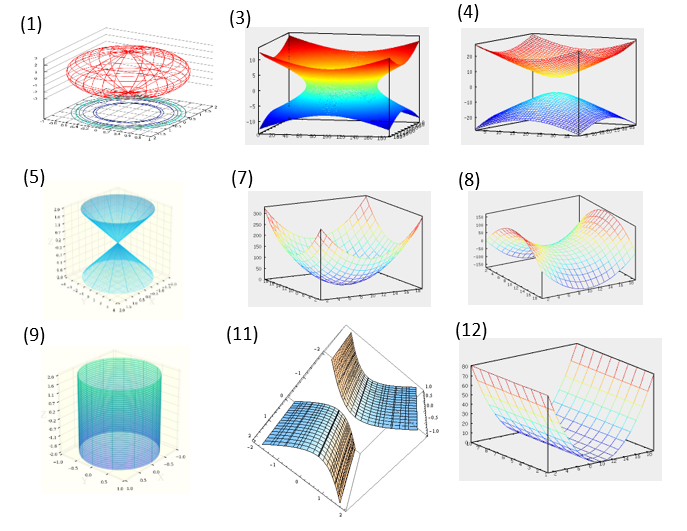
\includegraphics[width=1\textwidth]{П2П_1.PNG}
\end{center}







\part{Основы высшей алгебры}
\chapter{Комплексные числа.}

\section{Понятие комплексного числа. Арифметические операции с комплексными числами.}

$\bullet$ \textit{\textbf{Комплексным числом} называют выражение вида $z = a + bi$, где $a, b$ --- действительные числа, а $i$ --- символ, называемый \textbf{мнимой единицей}}.\\
\begin{examp}
	$i^2 = -1$, $z = 3 + 2i$ --- комплексное число, $a = 3, b = 2$.
\end{examp}\\\\
$a = Rez$ --- \textbf{действительная часть комплексного числа}.\\
$b = Imz$ --- \textbf{мнимая часть комплексного числа}.\\\\
$\bullet$ \textit{Комплексное число, у которого действительная часть равна нулю, называется \textbf{чисто мнимым}. Комплексное число, у которого мнимая часть равна нулю --- \textbf{действительное число}}.\\\\
$\bullet$ \textit{Пусть есть два комплексных числа $z_1 = a_1 + b_1i, z_2 = a_2 + b_2i$. Они называются \textbf{равными}, если их действительные и мнимые части равны ($a_1 = a_2, b_1 = b_2 \Rightarrow z_1 = z_2$)}.\\\\
$\bullet$ \textit{\textbf{Суммой двух компексных чисел $z_1$ и $z_2$} называется комплексное число $z = (a_1 + a_2) + (b_1 + b_2)i$ (т.е. складываются действительные и мнимые части)}.\\\\
\textbf{\textit{Свойства суммы комплексных чисел:}}
\begin{enumerate}
	\item $z_1 + z_2 = z_2 + z_1$ \textit{(коммутативность)}.
	
	\begin{Proof}
		$z_1 + z_2 = (a_1 + a_2) + (b_1 + b_2)i = (a_2 + a_1) + (b_2 + b_1)i = z_2 + z_1$. 
	\end{Proof}
	
	\item $(z_1 + z_2) + z_3 = z_1 + (z_2 + z_3)$ \textit{(ассоциативность)}.
	
	\item \textit{(Введение разности комплексных чисел) $z_1 - z_2 = (a_1 - a_2) + (b_1 - b_2)i$. Следует из суммы: $z + z_2 = z_1 \Rightarrow z_1 - z_2 = z$.}
\end{enumerate}
Введём произведение комплексных чисел: $z_1z_2 = (a_1 + b_1i)(a_2 + b_2i) = a_1a_2 + a_1b_2i + b_1a_2i - b_1b_2 = (a_1a_2 - b_1b_2) + (a_1b_2 + b_1a_2)i = z$ --- \textbf{произведение двух комплексных чисел $z_1$ и $z_2$}.\\\\
\textbf{\textit{Свойства произведения комплексных чисел:}}
\begin{enumerate}
	\item $z_1z_2 = z_2z_1$ \textit{(коммутативность)}.
	
	\item $(z_1z_2)z_3 = z_1(z_2z_3)$ \textit{(ассоциативность)}.
	
	\item $z_1(z_2 + z_3) = z_1z_2 + z_1z_3$ \textit{(дистрибутивность относительно сложения)}.
\end{enumerate}
$\bullet$ \textit{Пусть $z = a + bi$. Комплексное число $\overline{z} = a - bi$ называется \textbf{сопряжённым} комплексным числом к комплексному числу $z$ (равны действительные части, а мнимые отличаются на знак)}.\\\\
Введём деление комплексных чисел: $\dfrac{z_1}{z_2} = \dfrac{a_1 + b_1i}{a_2 + b_2i} = [\text{домножим на сопряженное знаменателю}] = \dfrac{(a_1 + b_1i)(a_2 - b_2)}{(a_2 + b_2i)(a_2 - b_2)} = \dfrac{(a_1 + b_1i)(a_2 - b_2i)}{a_2^2 + b_2^2}$\\
\begin{examp} Пусть
	$z_1 = 2 - 3i, z_2 = -3 + 7i$.\\
	$z_1 + z_2 = -1 + 4i;\\ z_1 - z_2 = 5 - 10i$;\\
	$z_1z_2 = (2 - 3i)(-3 + 7i) = -6 + 14i + 9i + 21 = 15 + 23i$;\\
	$\dfrac{z_1}{z_2} = \dfrac{2 - 3i}{-3 + 7i} = \dfrac{(2 - 3i)(-3-7i)}{(-3 + 7i)(-3 - 7i)} = \dfrac{-6 - 14i + 9i - 21}{9 + 49} = \dfrac{-27 - 5i}{58}.$
\end{examp}\\\\
\textbf{\textit{Свойства сопряжённых комплексных чисел:}}
\begin{enumerate}
	\item $z + \overline{z} = 2Rez = 2a; z - \overline{z} = 2iImz = 2bi$.
	
	\item $z = \overline{z} \Leftrightarrow z \in \mathbb{R}$.
	\begin{Proof}
		$\Rightarrow) z = \overline{z} \Rightarrow z - \overline{z} = 0 \Rightarrow 2iImz = 0 \Rightarrow Imz = 0 \Rightarrow z \in \mathbb{R}$
		
		$\Leftarrow) z \in \mathbb{R} \Rightarrow z = a, \overline{z} = a \Rightarrow z = \overline{z}.$
	\end{Proof}
	
	\item $\overline{z_1 + z_2} = \overline{z_1} + \overline{z_2}; \overline{z_1 - z_2} = \overline{z_1} - \overline{z_2}$.
	\begin{Proof}
		Пусть $z_1 = a_1 + b_1i, z_2 = a_2 + b_2i$. $z_1 + z_2 = (a_1 + a_2) + (b_1 + b_2)i. \overline{z_1 + z_2} = (a_1 + a_2) - (b_1 + b_2)i = (a_1 - b_1i) + (a_2 - b_2i) = \overline{z_1} + \overline{z_2}$. С вычитанием аналогично.
	\end{Proof}
	\item $\overline{z_1z_2} = \overline{z_1}\overline{z_2}$.
	\item $\overline{(\dfrac{z_1}{z_2})} = \dfrac{\overline{z_1}}{\overline{z_2}}$.
\end{enumerate}



\section{Извлечение корня из комлпексного числа.}
Пусть $z$ --- некоторое комплексное число.\\\\
$\bullet$ \textit{\textbf{Корнем $n$-ой степени из комплексного числа} $z$ называется число $z_0$ такое, что $z_0$ в степени $n$ равно Самому комплексному числу $z$. То есть $z_0^n = z$.}
\newtheorem*{t6_3_1}{Теорема}\begin{t6_3_1} Извлечение корня $n$-ой степени из комплексного числа $z = \rho e^{i\varphi}$ всегда возможно и, при $z\ne 0$, даёт
	ровно $n$ различных значений: $$z_k = \sqrt[n]{\rho}e^{i\frac{\varphi + 2\pi k}{n}},\ k=0,\dots,n-1,$$
	где $\sqrt[n]{\rho}$ --- действительное положительное число, $n$-ая степень которого равна $\rho$.
\end{t6_3_1}
\begin{examp}
	Извлечение квадратного корня из комплексного числа. \\Пусть $z = a + bi$, $z_0 = \sqrt{z}$, то есть $z_0^2 = z$, $z_0 = a_0 + b_0i$. \\Тогда $(a_0 + b_0i)^2 = a_0^2 + 2 a_0 b_0 i - b_0^2 = a + bi$. Следовательно, получаем систему$\begin{cases}
		a_0^2 - b_0^2 = a,\\
		2a_0b_0 = b;
	\end{cases}\Rightarrow\begin{cases}
		a_0^4 - 2 a_0^2 b_0^2 i - b_0^4 = a^2,\\
		4a_0^2b_0^2 = b^2;
	\end{cases}\Rightarrow (a_0^2 + b_0^2)^2 = a^2 + b^2\Rightarrow\begin{cases}
		a_0^2 - b_0^2 = a,\\
		a_0^2 + b_0^2 = \sqrt{a^2 + b^2};
	\end{cases}\Rightarrow\\\begin{cases}a_0^2 = \frac{1}{2}(a + \sqrt{a^2 + b^2}) > 0,\\
		b_0^2 = \frac{1}{2}(-a + \sqrt{a^2 + b^2}) > 0.
	\end{cases}$
\end{examp} 
	
	
	
	
	
	\chapter{Алгебраические структуры}
	\section{Бинарные отношения.}
	Пусть $X$ и $Y$ --- непустые множества.\\\\
	$\bullet$ \textit{Множество $X \times Y = \{ (x,y)\ |\ x\in X,\ y \in Y\}$ называется \textbf{декартовым произведением} $X$ на $Y$.}\\
\begin{examp}
		Пусть $X = \{1,2\}$, $Y = \{2, 3\}$. Тогда $X\times Y = \{(1,2), (1,3), (2,2), (2,3)\}$. В свою очередь $Y\times X = \{ (2,1), (3,1), (2,2), (3,2)\}$.
\end{examp}\\\\
	Возьмём $Y = X$.\\\\
	$\bullet$ \textit{Декартовое произведение $X^2 = X\times X = \{ (x,y)\ |\ x\in X,\ y \in X\}$ называется \textbf{декартовым квадратом}.}\\
	\begin{examp}
	Возьмём множество $X$ из предыдущего примера.\\ Тогда $X \times X = \{ (1,1), (1,2), (2,1), (2,2)\}$.
	\end{examp}\\\\
	$\bullet$ \textit{Любое подмножество декартового квадрата является \textbf{бинарным отношением}, определенным на $\sigma \subset X^2$.}\\
	\begin{examp}
		Если $(x,y)\in \sigma$, то $[\dfrac{x}{y} = \sigma]\Longleftrightarrow x\sigma y$.\\
	Если множество $L$ --- прямые, то $L^2$ --- пары прямых. Тогда если $\sigma = ||$ и $|| \subset L^2$, то $(\Delta_1, \Delta_2)\in || \Longleftrightarrow \Delta_1 || \Delta_2$.
	\end{examp}\\\\
	$\bullet$ \textit{Бинарное отношение $\sigma \subset X^2$ называется \textbf{отношением эквивалентности}, если выполняются условия}\begin{enumerate}
		\item $\forall x\in X\quad x\sigma x\ ((x,x) \in \sigma)$ --- \textit{\textbf{рефлексивность}}.
		\item $x \sigma y, y\sigma z\Rightarrow x \sigma z\ ((x,y) \in \sigma$ и $(y,z) \in \sigma \Rightarrow (x,z) \in \sigma)$ --- \textit{\textbf{транзитивность}}.
		\item $x \sigma y\Rightarrow y\sigma x\ ((x,y)\in \sigma\Rightarrow (y,x) \in \sigma)$ --- \textbf{\textit{симметричность}}.
	\end{enumerate}
	\textit{Обозначение: $\sim$ (например $x\sim y$)}.\\
	\begin{examp}
	Пусть $X = \{1,2,3\}$. Тогда\\
	$\sigma = \{(1,1)\}$ --- нет рефлексивности.\\
	$\sigma = \{(1,1), (2,2), (3,3), (1,2), (2,1), (1,3)\}$ --- нет симметричности.\\
	$\sigma = \{(1,1), (2,2), (3,3), (1,2), (2,1), (1,3), (3,1)\}$, $(2,1), (1,3) \Rightarrow (2,3) \in \sigma$ --- ?!, нет транзитивности.
	\end{examp}\\\\
	$\bullet$ \textit{Подмножество $\overline{x} = \{ x' \in X\ |\ x' \sim x\}$ множества $X$ при $x\in X$ называется \textbf{классом эквивалентности элемента $x$}. Любой элемент $x'\in \overline{x}$ называется \textbf{представителем класса $\overline{x}$}.}
	\newtheorem*{lem25_1}{Лемма}\begin{lem25_1}$x_1 \sim x_2 \Longleftrightarrow \overline{x}_1 = \overline{x}_2,\ x_1, x_2\in X$.\end{lem25_1}
	\begin{Proof}
		$\Rightarrow$) $x_1\sim x_2\Rightarrow $  возьмём произвольный $x \in \overline{x}_1\Rightarrow x\sim x_1, x_1\sim x_2 \Rightarrow x \sim x_2 \Rightarrow x\in \overline{x}_2 \Rightarrow \overline{x}_1 = \overline{x}_2$.\\\\
		$\Leftarrow)\ \overline{x_1} = \overline{x_2}.$ Возьмем $x_1 \in \overline{x_1}$ и $x_2\in \overline{x_2}\Rightarrow x_1 \in \overline{x_2}\Rightarrow x_1 \sim x_2$.
	\end{Proof}\\\\
	$\bullet$ \textit{Если $X$ представимо в виде объединения попарно непересекающихся подмножеств $(X = \bigcup x_i,\ x_i\cup x_j = \varnothing)$, то данное множество \textbf{разбивается на эти подмножества}.}
	\newtheorem*{th25_1}{Теорема}\begin{th25_1}Пусть на множестве $X$ задано бинарное отношение эквивалентности, тогда $X$ разбивается на непересекающиеся классы
		эквивалентности.
	\end{th25_1}
	\begin{Proof}
		$\forall x \in X, x \in \overline{x}\subset X, X = \bigcup\limits_{x\in X}\{x\}\subset \bigcup\limits_{x\in X}\overline{x}\subset X$. С другой же стороны $X = \bigcup\limits_{x\in X}\overline{x}$.\\\\
		Покажем, что два класса эквивалентности $\overline{x}_1$ и $\overline{x}_2$ не пересекаются или совпадают ($\overline{x}_1 = \overline{x}_2$ или $\overline{x}_1\cap \overline{x}_2 = \varnothing$):\\
		Пусть $\overline{x}_1\cap \overline{x}_2 \ne \varnothing$. Тогда найдется $x \in \overline{x}_1 \in \overline{x}_2\Rightarrow x\in \overline{x}_1, x\in \overline{x}_2\Rightarrow x\sim x_1, x\sim x_2 \Rightarrow [x_1\sim x, x_2\sim x\Rightarrow x_1\sim x_2]\Rightarrow$ если $x_1 \sim x_2$, то $\overline{x_1} = \overline{x_2}$ по лемме.
	\end{Proof}\\\\
	$\bullet$ \textit{Бинарное отношение $\sigma$ на множестве $X$ называется \textbf{отношением порядка}, если выполняются условия}\begin{enumerate}
		\item $\forall x\in X\quad x\sigma x$ --- \textit{\textbf{рефлексивность}}.
		\item $x \sigma y, y\sigma z\Rightarrow x \sigma z$ --- \textit{\textbf{транзитивность}}.
		\item $x \sigma y\Rightarrow x = y$ --- \textbf{\textit{антисимметричность}}.
	\end{enumerate}
	\textit{Обозначение: $\leqslant$ (например $x\leqslant y$)}.\\
\begin{examp}
		Пусть $X = \{1,2\}$. Тогда\\
	$\sigma = \{ (1,1), (2,2), (1,2), (2,1)\}$ --- нет антисимметричности.\\
	$\sigma = \{(1,1), (2,2), (1,2)\}$ --- отношение порядка.
\end{examp}
	
	
	
	
	
		\section{Отображения.}
	Пусть $X$, $Y$ --- некоторые непустые множества.\\\\
	$\bullet$ \textit{Определено однозначное \textbf{отображение} множества $X$ на множество $Y$, если каждому элементу из множества $X$ соответствует единственный элемент из множества $Y$. Обозначение: $f$: $x$ $\rightarrow$ $Y\ x\in X$ или $f:x\mapsto y\ f(x) = y$}.\\\\
	$\bullet$ \textit{Если отображение f элемент x ставит в соответствие элементу y, то говорят, что $y$ --- \textbf{образ} элемента x, а $x$ --- \textbf{прообраз} элемента y. Обозначение: $\{x\in X\ |\ f(x) = y\}$ --- полный прообраз элемента $y$;  $\{f(x)\ |\ \forall x\in X \} = Imf = f(X)\subset Y$ --- образ $x$ при $f$}. \\\\
	$\bullet$ \textit{Отображение $f: X\rightarrow Y$ называется \textbf{инъективным}, если $x_1$ $\not=$ $x_2$ $\Rightarrow$ \\ $f(x_1)$ $\not=$ $f(x_2)$\quad $\forall x_1, x_2$ $\in$ $X$}.\\\\
	$\bullet$ \textit{Отображение $f: X\rightarrow Y$ называется \textbf{сюръективным}, если $\forall$$y$ $\in$ $Y$  $\exists$$x$ $\in$ $X$ : $f(x)$ = $y$}.\\\\
	$\bullet$ \textit{Отображение $f: X\rightarrow Y$ называется \textbf{биективным}, если оно инъективно и сюръективно} \textit{(взаимнооднозначное соответствие)}.\\\\
	$\bullet$ \textit{Два отображения $f$: $X$ $\rightarrow$ $Y$ и $g$: $X'$ $\rightarrow$ $Y'$ называются \textbf{равными}, если $X$ = $X'$}, \\ \textit{$Y$ = $Y'$ и $\forall x$ $\in$ $X$ $f(x)$ = $g(x)$.}\\\\
	Пусть $f$: $X$ $\rightarrow$ $Y$ --- некоторое отображение. $X'$ $\subset$ $X$. Тогда \\\\
	$\bullet$ \textit{Отображение $g$: $X' \rightarrow Y'$ называется \textbf{ограничением (сужением) отображения} $f$ на множестве $X'$, если $\forall x$ $\in$ $X'$ $g(x) = f(x)$. Обозначение: $f|_\textit{X'}$. Само же отображение $f:X\rightarrow Y$ называется \textbf{продолжением отображения} $g$ на множестве $X$.}\\\\
	Пусть $f$: $X$ $\rightarrow$ $Y$ и $g$: $Y$ $\rightarrow$ $Z$. Тогда\\\\
	$\bullet$ \textit{Отображение $g$ $\circ$ $f$ : $X$ $\rightarrow$ $Z$ которое работает так, что $\forall x$ $\in$ $X$ $(g \circ f)(x)$ = $g(f(x))$, называется \textbf{композицией отображений} $g$ и $f$.}\\
	\begin{examp} Пусть $f(x) = sinx,\ g(x) = x^2 + x + 1$. Тогда\\
		$(g\circ f)(x) = g(f(x)) = g(sinx) = sin^2 x + sinx + 1;\\
		(f\circ g)(x) =f(g(x)) = f(x^2 + x + 1) = sin(x^2 + x + 1).$\\
		Из полученного выше следует, что $f\circ g \not= g\circ f$.
	\end{examp}\\\\
	Композиция отображений обладает свойством \textbf{ассоциативности}, то есть выражение \\$(h\circ g)\circ f = h\circ (g\circ f)$ верно. Докажем это:\\
	$((h\circ g)\circ f)(x) = (h\circ g)(f(x)) = h(g(f(x)))$;\\
	$(h\circ(g\circ f))(x) = h((g\circ f)(x)) = h(g(f(x)))$.
	\newtheorem*{t6_2}{Теорема}\begin{t6_2} Пусть $f$: $X$ $\rightarrow$ $Y$, $g$: $Y$ $\rightarrow$ $Z$ и $h = g \circ f$. Тогда
		\begin{enumerate}
			\item если $f$ и $g$ инъективны, то $h$ инъективно;
			\item если $f$ и $g$ сюръективны, то $h$ сюръективно;
			\item если $f$ и $g$ биективны, то $h$ биективно.
		\end{enumerate}
	\end{t6_2} \begin{Proof} \begin{enumerate}
			\item Пусть $f$ и $g$ --- инъекции, тогда $\forall x_1, x_2$ $\in$ $X$, $x_1$ $\not=$ $x_2$ $\Rightarrow$ $f(x_1)$ $\not=$ $f(x_2)$, $g(f(x_1)) \not= g(f(x_2))$ $\Rightarrow$ $h$ инъективно, так как $(g\circ f)(x_1) = g(f(x_1))$ = $h(x_1)$, $(g\circ f)(x_2) = g(f(x_2))$ = $h(x_2)$, $h(x_1) \not= h(x_2)$.
			\item Пусть $f$ и $g$ --- сюръекции. Тогда, т.к. $g$ --- сюръекция $\forall z \in Z \exists y$ $\in$ $Y : g(y) = z$. А так как $f$ --- сюръекция, то  $\forall y \in Y$ $\exists x$ $\in$ $X : f(x) = y$ $\Rightarrow$ $\forall z$ $\in$ $Z$ $\exists x$ : $h(x) = (g \circ f)(x) = g(f(x)) = g(y) = z$ --- сюръекция.
			\item Биективность вытекает из двух предыдущих пунктов.
	\end{enumerate} \end{Proof}\\
	$\bullet$ \textit{Отображение $e_x : X$ $\rightarrow$ $X$ такое, что $\forall x$ $\in$ $X$ $e_x(x) = x$ называется \textbf{тождественным отображением} множества $X$}.\\\\
	Пусть $f$ : $X$ $\rightarrow$ $Y$ --- некоторое отображение. \\\\
	$\bullet$ \textit{Отображение $g$ : $Y$ $\rightarrow$ $X$ называется \textbf{обратным} для отображения $f$, если $g \circ f$ = $e_x$, $f \circ g$ = $e_y$.}\\
	\begin{examp}
		Пусть $f(x) = lnx, g(x) = e^x$. Тогда $f(g(x)) = f(e^x) = lne^x = x = g(f(x)) = e^{lnx} = x.$
	\end{examp}
	\newtheorem*{t6_2_2}{Теорема}\begin{t6_2_2} Отображение $f$ : $X$ $\rightarrow$ $Y$ имеет обратное $\Longleftrightarrow$ оно биективно.
	\end{t6_2_2} 
	
	
	
	
	\section{Бинарная алгебраическая операция.}
	Пусть $X$ --- некоторое непустое множество.\\\\
	$\bullet$ \textit{Отображение $f$ : $X^2$ $\rightarrow$ $X$, действующее так, что $(a,b) \mapsto c \forall a,b \in X^2, c \in X$ называется \textbf{бинарной алгебраической операцией.} \\ Обозначается $f$ : $(a,b)$ $\mapsto$ $c$ или $f(a,b) = c$}.\\\\
	Для произвольной алгебраической операции $a * b = c$, где $*$ --- символ символ (они могут выглядеть по-разному: $+, -, \cdot$ и так далее).\\\\
	$\bullet$ \textit{Множество $X$ c определенной на нем алгебраической операцией $*$ является \textbf{алгебраической структурой}. Обозначается $(X, *)$}.\\
	\begin{examp}
		$(N,\cdot), (N,+)$ --- две разные алгебраические структуры.
	\end{examp}\\\\
	$\bullet$ \textit{Алгебраическая операция $*$ называется} \begin{enumerate}
		\item \textit{\textbf{ассоциативной,} если $(x*y)*z = x*(y*z)$ $\quad\forall x, y, z\in X$;}
		\item \textit{\textbf{коммутативной,} если $x*y = y*x$ $\quad\forall a, b$.}
	\end{enumerate}\begin{examp}
		Для структуры $(R,+)$ операция $+$ ассоциативна, т.к. $a + (b+c) = (a+b) + c$. Для структуры $(R, -)$ операция $-$" не ассоциативна, т.к. $a-(b-c)\ne (a-b)-c$.\\
		Также операция $+$ является коммутативной в отличие от операции $-$.
	\end{examp}\\\\
	$\bullet$ \textit{Элемент $n$ $\in$ $X$ называется \textbf{нейтральным} элементом в $X$ относительно операции $* \Longleftrightarrow n * x = x * n = x\quad\forall x$ $\in$ $X$.}\\
	\begin{examp}
		Рассмотрим несколько структур их нейтральные элементы:\\
		$(R, +)$, $n = 0$\quad$x+0 = 0 + x = x$;\\
		$(R, \cdot)$, $n = 1$\quad$x\cdot1 = 1\cdot x= x$;\\
		$(R, -)$, $\not\exists n$\quad$x-n \not= n-x \not= x$.
	\end{examp}
	\newtheorem*{t6_3}{Теорема}\begin{t6_3}Структура $(X, *)$ имеет не больше одного нейтральгого элемента. \end{t6_3} 
	\begin{Proof} От противного. Пусть $\exists n_1, n_2 : n_1\not= n_2$. Тогда $n_1 * n_2 = n_1$, $n_2 * n_1 = n_2$ $\Rightarrow$ $n_1 = n_2$, что является противоречием. \end{Proof} \\\\
	Пусть $(X, *)$, $\exists n \in X$.\\\\
	$\bullet$ \textit{Элемент $x'\in X$ называется \textbf{симметричным} для элемента $x\in X$ относительно операции $*$, если $x' * x = x * x' = n$.}
	\newtheorem*{t6_3_2}{Теорема}\begin{t6_3_2} Если в $(X, *)$ операция $*$ ассоциативна и $\exists n \in X$, то $\forall a\in X$ может существовать не более одного симметричного элемента.  \end{t6_3_2} 
	\begin{Proof}
		От противного. Пусть $\exists a \in X :  \exists a', a''$ Тогда $a' * a$ = $a * a'$ = $n$, $a'' * a$ = $a * a''$ = $n$ $\Rightarrow$ $a' = a' * n = a' * (a * a'') = (a' * a) * a'' = n * a'' = a''$ $\Rightarrow$ $a' = a''$. \end{Proof} \\\\
	Рассмотрим некоторые операции и их характеристику:\begin{center}
		\begin{tabular}{|c|c|c|}
			\hline
			Операция & Аддитивная запись & Мультипликативная запись  \\
			\hline
			Знак & $+$ & $\cdot$ \\
			Название & сложение & умножение \\
			Результат & сумма & произведение \\
			Нейтральный элемент & $0$ & $1$ \\
			Симметричный элемент & $-x$ (противоположный) & $x^{-1}$ (обратный) \\
			\hline
		\end{tabular}
	\end{center}
	
	
	
	\chapter{Многочлены}
	\section{Кольцо многочленов.}
	Пусть $P$ --- некоторое поле.\\\\
	$\bullet$ \textit{Выражение вида $a_{n}x^n + a_{n-1}x^{n-1} + \ldots + a_1x + a_0$, где $\alpha_i \in P, i = \overline{0,n}$ называется \textbf{многочленом над полем $P$}. Обозначение: $f(x)$. При этом элементы $a_i$ называются \textbf{коэффициентами многочлена}, $x$ --- \textbf{переменными многочлена}, $a_ix^i$ --- \textbf{членом многочлена}. Число $n$ называется \textbf{степенью многочлена}, если $a_n \ne 0$, а $a_i = 0 \forall i > n$. Обозначение: $n = deg\ f(x)$. При этом коэффициент $a_n$ называется \textbf{старшим} коэффициентом, а $a_0$ --- свободным членом.} \\
	\begin{examp}
		Пусть $f(x) = 5x^2 + 3x + 7$. Тогда $deg\ f(x) = 2$, $a_2 = 5$, $a_1 = 3$, $a_0 = 7$.
	\end{examp}\\\\
$\bullet$ \textit{Если все коэффициенты многочлена равны нулю, то многочлен называется \textbf{нулевым многочленом}. Степень нулевого многовлена не определена.}\\\\
$\bullet$ Два многочлена $f(x)$ и $g(x)$ называются равными $\Longleftrightarrow deg\ f(x) = deg\ g(x)$ и равны коэффициенты при соответствующих степенях $x$.\\\\
Множество всех многочленов над полем $P$ от переменной $x$ обозначается как $P[x]$.\\ \begin{examp}
	Множества $\mathbb{R}[x]$ и $\mathbb{C}[x]$ --- множества всех многочленов от переменной $x$ с действительными и комплексными коэффициентами соответственно.
\end{examp}\\\\
Рассмотрим два многочлена:\\
$f(x) = a_nx^n + \ldots + a_1 x + a_0,\ deg\ f(x) = n,\ a_n \ne 0,$\\
$g(x) = b_kx^k +\ldots + b_1x + b_0,\ deg\ g(x) = k,\ n\geqslant k.$\\\\
$\bullet$ \textit{\textbf{Суммой многочленов} $f(x)$ и $g(x)$ называется многочлен вида $(f+g)(x) = c_nx_n + \ldots + c_1x + c_0,\ c_i = a_i + b_i \forall i = \overline{0,n},\ c_i = a_i \forall i = \overline{k+1, n}.$\\
	$deg\ (f+g)(x) \leqslant max\{deg\ f(x),\ deg\ g(x)\}.$}\\\\
$\bullet$\textit{ \textbf{Произведением многочленов} $f(x)$ и $g(x)$ называется многочлен вида $f(x)\cdot g(x) = d_{n+k}x^{n+k} + \ldots + d_1x + d_0,\ d_i = \sum_{s+l=i}a_sb_l,\ i = \overline{0,n+k}.$\\
$deg\ (f(x)\cdot g(x)) = deg\ f(x) + deg\ g(x),\ d_{n+k} = \sum_{s+l=n+k} a_sb_l = \underset{\ne0}{a_n}\underset{\ne 0}{b_k}.$}
\newtheorem*{th29}{Теорема}\begin{th29}
	Множество $P[x]$ является ассоциативным, коммутативным кольцом с единицей относительно операции сложения и умножения многочленов.
\end{th29}\begin{Proof} Пусть $f(x), g(x) \in P[x]$. Тогда $f(x) + g(x) \in P[x], f(x)\cdot g(x)\in P[x]$.\\\\
Рассмотрим множество $P[x]$ относительно операции $+$ и докажем аксиомы кольца.\begin{enumerate}
	\item $f(x) + g(x) = (a_n + b_n)x^n + \ldots + (a_1 + b_1) x + (a_0 + b_0) = (b_n + a_n)\cdot x^n + \ldots + (b_1 + a_1)x + (b_0 + a_0) = g(x) + f(x).$ Значит, операция коммутативна.
	\item $(f(x) + g(x)) + h(x) = f(x) + (g(x) + h(x))$. Значит, операция ассоциативна.
	\item Пусть $n(x) = 0$. Тогда $f(x) + 0(x) = (a_n + 0)x^n + (a_1 + 0)x + a_0 + 0 = f(x).$ Значит, суещствует нейтральный элемент.
	\item $f(x) = a_nx^n + \ldots + a_1 x + a_0.\\
	-f(x) = -a_nx^n - \ldots - a_1 x + a_0\Rightarrow f(x) + (-f(x)) = 0$. Значит, для произвольного элемента суещствует обратный.
	\item $(f(x) + g(x))h(x) = f(x)h(x) + g(x)h(x) \Rightarrow P[x]$ --- кольцо. Проверим операцию умножения: \\$f(x)\cdot g(x) = g(x)\cdot f(x);$\\
	$(f(x)\cdot g(x))h(x) = f(x) \cdot (g(x)\cdot h(x));$\\
	$f(x) = 1 \Rightarrow f(x)g(x) = g(x)$. Обратного элемента не существует, следовательно множество является кольцом, но не является полем.
\end{enumerate}
\end{Proof}\\
\textbf{\textit{Свойства кольца многочленов:}}\begin{enumerate}
	\item \textit{В кольце многочленов не существует делителей нуля.}
	\begin{Proof}
		Пусть $f(x) \ne 0$, $a \ne 0$, $g(x) \ne 0$, $b\ne 0$. Тогда $f(x)\cdot g(x) \ne 0$, $a\cdot b\ne 0$.
	\end{Proof}
	\item \textbf{Закон сокращения:}
	$f(x)h(x) = g(x)h(x)\Rightarrow f(x) = g(x)$.
	\begin{Proof}
		$f(x)h(x) - g(x)h(x) = 0 \Rightarrow \underset{\ne0}{h(x)}(f(x) - g(x)) = 0\Rightarrow f(x) - g(x) = 0 \Rightarrow $ так как в кольце нет делителей нуля, $f(x) = g(x).$
	\end{Proof}
	\item $\exists f^{-1} \Longleftrightarrow f(x) = a \ne 0$.
	\begin{Proof}
		$\Rightarrow)$ Пусть $\exists f^{-1}(x) : f^{-1}(x)\cdot f(x) = 1$.\\
		$deg\ (f^{-1}(x)\cdot f(x)) = deg\ f^{-1}(x) + deg\ f(x) = 0\Rightarrow deg\ f(x) = 0\Rightarrow f(x) = a$.\\\\
		$\Leftarrow)$ Пусть $f(x) = a \ne 0$. Тогда $f^{-1}(x) = \dfrac{1}{a}$. 
	\end{Proof}
\end{enumerate}
	
	
	
	
	
	\chapter{Матрицы и определители}
	\section{Определитель матрицы.}
	
	\textit{Пусть дана квадратная матрица $A \in P_{n, n}$. Число $det A = \sum\limits_{\alpha \in \delta_n} (-1)^{\varepsilon(\alpha)}a_{1\alpha_1} \cdot a_{2\alpha_2} \cdot \dots \cdot a_{n\alpha_n}$ называется \textbf{определителем матрицы $A$}}.\\
	\begin{examp}\\
	1) $n = 1, A = (a_{11}), \delta_1 = {(1)}$\\
	2) $n = 2, A =  \begin{pmatrix}
		a_{11}& a_{12}\\
		a_{21}& a_{22}
	\end{pmatrix}, \delta_2 = {(1, 2), (2, 1)}$\\
	3) $n = 3, A =  \begin{pmatrix}
		a_{11}& a_{12} & a_{13}\\
		a_{21}& a_{22} & a_{23}\\
		a_{31} & a_{32} & a_{33}
	\end{pmatrix}, \delta_2 = {(1, 2, 3), (1, 3, 2), (2, 1, 3), (2, 3, 1), (3, 2, 1), (3, 1, 2)}$. $det A = a_{11}a_{22}a_{33} - a_{12}a_{21}a_{33} - a_{11}a_{23}a_{32} + a_{12}a_{23}a_{31} - a_{13}a_{22}a_{31} + a_{13}a_{21}a_{32}$.\\\\
	У диагональной матрицы определитель равен произведению диагональных элементов, а определитель единичной матрицы равен 1.
	\end{examp}\\\\
	\textbf{\textit{Свойства определителя:}}
	\begin{enumerate}
		\item\textit{ Если матрица $B$ получена из матрицы $A$, поменяв местами две строки, то $det B = -det A$.}
		\begin{Proof}
			Поменяем строки с номерами $s, k$ и $s < k$. Тогда $\forall j: a_{sj} = b_{kj}, a_{kj} = b_{sj}, a_{ij} = b_{ij} \forall j \ne s, i \ne k$.\\\\
			По определению $det A = \sum\limits_{\alpha \in \delta_n} (-1)^{\varepsilon(\alpha)}a_{1\alpha_1} \cdot ... \cdot a_{s\alpha_s}\cdot ... \cdot a_{k\alpha_k} \cdot a_{n\alpha_n} = \sum\limits_{\alpha \in \delta_n} (-1)^{\varepsilon(\alpha)}b_{1\alpha_1} \cdot ... \cdot b_{k\alpha_s}\cdot ... \cdot b_{s\alpha_k} \cdot b_{n\alpha_n} = \sum\limits_{\alpha \in \delta_n} (-1)^{\varepsilon(\alpha_1...\alpha_k...\alpha_s...\alpha_n)}b_{1\alpha_1} \cdot ... \cdot b_{s\alpha_s}\cdot ... \cdot b_{k\alpha_k} \cdot b_{n\alpha_n} = -det B$ (т.е. поменялась чётность перестановки).
		\end{Proof} 
		\item \textit{Если матрица содержит две одинаковые строки, то её определитель равен нулю.}
		\begin{Proof}
			$det A = - det A$ (по первому свойству).
		\end{Proof}
		\item\textit{ Если любую строки матрицы $A$ умножить на скаляр $\lambda \in P$, то получится матрица $B$: $det B = \lambda det A$.}
		\begin{Proof}
			$A = (a_{ij}) \in P_{n,n}, B = (b_{ij}) \in P_{n, n}$. Пусть мы умножили $k$-ю строку матрицы $A$ и получили матрицу $B \Rightarrow b_{kj} = \lambda a_{kj} \forall j = \overline{1, n}, b_{ij} = a_{ij} \forall i \ne k$.\\\\
			Тогда $det B = \sum\limits_{\alpha \in \delta_n} (-1)^{\varepsilon(\alpha)}b_{1\alpha_1} \cdot ... \cdot b_{k\alpha_k}  \cdot  ... \cdot b_{n\alpha_n} = $ [заменим на элементы матрицы $A$] $= \sum\limits_{\alpha \in \delta_n} (-1)^{\varepsilon(\alpha)}a_{1\alpha_1} \cdot ... \cdot \lambda a_{k\alpha_k} \cdot  ... \cdot a_{n\alpha_n} = \lambda\sum\limits_{\alpha \in \delta_n} (-1)^{\varepsilon(\alpha)}a_{1\alpha_1} \cdot ... \cdot a_{k\alpha_k}  \cdot  ... \cdot a_{n\alpha_n} = \lambda det A$.
		\end{Proof}
		\newtheorem*{cor41_1}{Следствие}\begin{cor41_1} Если матрица содержит нулевую строку, то её определитель равен нулю.
		\end{cor41_1}
		\newtheorem*{cor41_2}{Следствие}\begin{cor41_2} $\forall A \in P_{n,n}: det(\lambda A) = \lambda^n detA$.
		\end{cor41_2}
		\newtheorem*{cor41_3}{Следствие}\begin{cor41_3} Если матрица содержит две пропорциональные строки, то её определитель равен нулю.
		\end{cor41_3}
		\item $\Delta = \begin{vmatrix}
			a_{11}& a_{12} & ... & a_{1n}\\
			... \\
			a'_{k1} + a''_{k1} & a_{k2} & ... &a_{kn}\\
			... \\
			a_{n1} & a_{n2} & ... & a_{nn}
		\end{vmatrix} = \begin{vmatrix}
			a_{11}& a_{12} & ... & a_{1n}\\
			... \\
			a'_{k1} & a_{k2} & ... &a_{kn}\\
			... \\
			a_{n1} & a_{n2} & ... & a_{nn}
		\end{vmatrix} + \begin{vmatrix}
			a_{11}& a_{12} & ... & a_{1n}\\
			... \\
			a''_{k1} & a_{k2} & ... &a_{kn}\\
			... \\
			a_{n1} & a_{n2} & ... & a_{nn}
		\end{vmatrix} = \Delta_1 + \Delta_2$
		\begin{Proof}
			$\Delta = \sum\limits_{\alpha \in \delta_n} (-1)^{\varepsilon(\alpha)}a_{1\alpha_1} \cdot ... \cdot (a'_{k1} + a''_{kn}) ...  \cdot a_{n\alpha_n} = \sum\limits_{\alpha \in \delta_n} (-1)^{\varepsilon(\alpha)}a_{1\alpha_1} \cdot ... \cdot a'_{k1} ...  \cdot a_{n\alpha_n} + \sum\limits_{\alpha \in \delta_n} (-1)^{\varepsilon(\alpha)}a_{1\alpha_1} \cdot ... \cdot a''_{kn} ...  \cdot a_{n\alpha_n} = \Delta_1 + \Delta_2$.
		\end{Proof} 
		\item \textit{Определитель матрицы не изменится, если к любой его строке прибавить другую, умноженную на произвольный элемент поля $P$.}
		\begin{Proof}
			$A = (a_{ij} \in P_{n,n} \lambda \in P) \Rightarrow det B =  \begin{pmatrix}
				a_{11}& a_{12} & \dots & a_{1n}\\
				\dots & \dots & \dots & \dots \\
				a_{k1} + \lambda a_{s1} & a_{k2} + \lambda a_{s2} & \dots &a_{kn} + \lambda a_{sn}\\
				\dots & \dots & \dots & \dots \\
				a_{n1} & a_{n2} & \dots & a_{nn}
			\end{pmatrix}.$
			
			$det B =  \begin{vmatrix}
				a_{11}& a_{12} & ... & a_{1n}\\
				... \\
				a_{k1} + \lambda a_{s1} & a_{k2} + \lambda a_{s2} & ... &a_{kn} + \lambda a_{sn}\\
				... \\
				a_{n1} & a_{n2} & ... & a_{nn}
			\end{vmatrix} = [по свойству 4] =  \begin{vmatrix}
				a_{11}& a_{12} & ... & a_{1n}\\
				... \\
				a_{k1} & a_{k2} & ... &a_{kn} \\
				... \\
				a_{n1} & a_{n2} & ... & a_{nn}
			\end{vmatrix} + \begin{vmatrix}
				a_{11}& a_{12} & ... & a_{1n}\\
				... \\
				\lambda a_{s1} & \lambda a_{s2} & ... &\lambda a_{sn}\\
				... \\
				a_{n1} & a_{n2} & ... & a_{nn}
			\end{vmatrix}.$ Второй определитель равен нулю, т.к. имеет 2 пропорциональные строки.
		\end{Proof}
		
		\item \textit{Определитель матрицы при транспонировании не меняется.}
		\begin{Proof} $A = (a_{ij}), A^T = B = (b_{ij}), a_{ij} = b_{ji} \forall i, j = \overline{1, n}$.\\\\
			$det A = \sum\limits_{\alpha \in \delta_n} (-1)^{\varepsilon(\alpha)}a_{1\alpha_1} \cdot ... \cdot a_{\alpha_nn} = \sum\limits_{\alpha \in \delta_n} (-1)^{\varepsilon(\alpha)}b_{\alpha_11} \cdot ...  \cdot b_{\alpha_nn}$.\\\\
			Каждая перестановка множителей порождает транспозицию в перестановке, состоящей из индексов $\Rightarrow$ переупорядочивание элементов в произведении влечёт за собой цепочку транспозиций, переводящих перестановки, притом чётность этих перестановок будет совпадать $\Rightarrow$ $det A = \sum\limits_{\alpha \in \delta_n} (-1)^{\varepsilon(\beta)}b_{1\beta_1} \cdot ...  \cdot b_{n\beta_n} = det B$. \end{Proof}
	\end{enumerate}
	\newtheorem*{cor41_4}{Следствие}\begin{cor41_4}
		Все свойства строк матрицы равносильны и для столбцов
	\end{cor41_4}
	
	
	
	
	
	
	
	
	
	\section{Алгоритм Евклида. Основная теорема арифметики. Китайская теорема об остатках.}
	
	Пусть $a, b \in z, b \ne 0$. Тогда любое число можно представить в виде: $a = bq + r, 0 \leq r < |b|$. К примеру, $-23 = 5(-5) + 2$. Остаток $(r)$ - число неотрицательное. Притом, такое представление является единственным (доказать можно от противного).
	
	\textit{\textbf{Число $b$ делит число $a$}, если $a = bq$ (т.е. остаток равен нулю).}
	
	Если число $b$ делит число $a$, то принято обозначать это следующим образом: $b | a$.\\\\
	\textbf{\textit{Свойства делимости:}}
	\begin{enumerate}
		\item $a | b, b | c \Rightarrow a | c$
		\begin{Proof}
			$b | c \Rightarrow c = bq_1.\ a | b \Rightarrow b = aq_2 \Rightarrow c = aq_1q_2 = aq$.
		\end{Proof}
		\item $a | b \Rightarrow a | bc \forall c \in Z$
		\begin{Proof}
			$a | b \Rightarrow b = aq_1 \Rightarrow bc = aq_1c = aq \Rightarrow a | bc$.
		\end{Proof}
		
		\item $c | a,\ c | b \Rightarrow c|(a + b)$
		\begin{Proof}
			$c | a \Rightarrow a = cq_1,\ c | b \Rightarrow b = cq_2 \Rightarrow (a + b) = c(q_1 + q_2) = cq$.
		\end{Proof}
	\end{enumerate}
	$\bullet$ \textit{Натуральное (целое положительное) число называется \textbf{простым}, если оно делится только на себя и единицу. Единица - не простое число.}\\\\
	$\bullet$ \textit{Пусть $d | a$ и $d | b$, тогда число $d$ называется \textbf{общим делителей чисел $a, b$}.}\\\\
	$\bullet$ \textit{Общий делитель, который делится на любой другой общий делитель, называется \textbf{наибольшим общим делителем (НОД)}}.\\\\
	$\bullet$ \textit{Если НОД(a, b) = 1, то эти числа называются \textbf{взаимно простыми}}.\\\\
	Выведем алгоритм нахождения НОД двух чисел. Пусть $a, b \in Z, a > b$. $a = bq_1 + r_1, 0 < r_1 < b$. НОД($a, b$) = НОД($b, r_1$).\\
	$d|a, d|b \Rightarrow r_1 = a - bq_1 \Rightarrow d | r_1, d|b$\\
	$d|b, d|r_1 \Rightarrow a = bq_1 + r_1 \Rightarrow d | a, d|b$\\
	НОД($a, b$) = НОД($b, r_1$) = НОД=($r_1, r_2$) = НОД($r_2, r_3$) = ... = НОД($r_{n-1}, r_n$).\\
	Таким образом, получили \textbf{алгоритм Евклида} нахождения НОД двух чисел. Проделываем его до момента, пока не получим нулевой остаток: последний ненулевой остаток будет являться НОДом.\\\\
	Любое натуральное число, не равное 1, можно представить в виде произведения простых чисел следующим образом: $a = p_1^{\alpha_1} \cdot ... \cdot p_k^{\alpha_k},\quad p_i \ne p_j\quad \forall i \ne j,\quad i, j = \overline{1, k}$.\\\\
	К примеру, $600 = 2^2 \cdot 3 \cdot 5^5$.\\\\
	$\bullet$ \textit{Если $a|c, b|c$, то $c$ называется \textbf{общим кратным} этих чисел.}\\\\
	$\bullet$ \textit{Пусть $m \in N$. Говорят, что \textbf{число $a$ сравнимо с числом $b$ по модулю $m$}, если разность $a - b$ делится на $m$. Обозначение: $a \equiv b(mod m) \Leftrightarrow m | (a - b)$}.\\\\
	\textbf{\textit{Свойства сравнений:}}
	\begin{enumerate}
		\item $a \equiv a (mod m)$ --- \textit{рефлексивность}.
		
		\item $a \equiv b(mod m), b \equiv c (mod m) \Rightarrow a \equiv c(mod m)$ --- \textit{транзитивность}.
		
		\item $a \equiv b(mod m) \Rightarrow b = a(mod m)$ --- \textit{симметричность}.
	\end{enumerate}
	Рассмотрим систему сравнений 
	$\begin{cases}
		x \equiv b_1 (mod m_1), \\
		\dotfill \\
		x \equiv b_k (mod m_k).
	\end{cases}$\\\\
	$\bullet$ \textit{Систему сравнений называют \textbf{совместной}, если она имеет хотя бы одно решение}.\\\\
	$\bullet$ \textit{Система сравнений называется \textbf{приведённой}, если числа $m_1, ..., m_k$ попарно взаимно просты.}\\\\
	\newtheorem*{th45_1}{Теорема (Китайская теорема об остатках)}\begin{th45_1}Приведённая система сравнений всегда совместна и равносильна сравнению $x \equiv b_1x_1\dfrac{m}{m_1} + ... + b_kx_k\dfrac{m}{m_k} (mod m)$, где $m = m_1 \cdot ... \cdot m_k, x_i$ --- произвольное решение сравнения $\dfrac{m}{m_i}x \equiv 1(mod m_i)$.
	\end{th45_1}
\end{document}